\documentclass{article}
\usepackage[utf8]{inputenc}
\usepackage{amsmath}
\usepackage{amsfonts}
\usepackage{graphicx}
\usepackage{amssymb}
\usepackage{amsthm}
\usepackage{float}
\usepackage{tikz}
\usepackage{mlmodern}
\usepackage{subfig}
\usepackage{pgfornament}
\usepackage{graphicx}
\usepackage{bm}
\usepackage{hyperref}
\usepackage[some]{background}
\usepackage[T1]{fontenc}
\usepackage[left=2.5cm,right=2.5cm]{geometry}
\usepackage[linesnumbered,ruled]{algorithm2e}
\usepackage{hyperref, xurl}
\usepackage{qrcode}
\usepackage{authblk} % for author info
\usepackage{svg}
\usepackage{listings}
\usepackage{epigraph} % used for the quotes

\usepackage[sorting=none]{biblatex}
\addbibresource{references.bib}

\newcommand{\maniflow}{\texttt{maniflow}}
\newcommand{\code}[1]{\texttt{#1}} % inline code setting
\renewcommand{\lstlistingname}{Code}

\definecolor{codebg}{RGB}{230,230,230}
\lstset {
    breakatwhitespace=false,         % sets if automatic breaks should only happen at whitespace
    breaklines=true,                 % sets automatic line breaking
    captionpos=b,                    % sets the caption-position to bottom
    tabsize=4,
    %showstringspaces=false,
    numbers=left,                    % where to put the line-numbers; possible values are (none, left, right)
    numbersep=2pt,                   % how far the line-numbers are from the code
    numberstyle=\tiny, % the style that is used for the line-numbers
    %upquote=true,
    backgroundcolor = \color{codebg},
    basicstyle=\small\ttfamily, % basic font setting
    emph={int,char,double,float,unsigned,void,bool},
    %emphstyle={\color{blue}},
    escapechar=\&,
    columns=fixed
}

\usepackage{collectbox}

\makeatletter
\newcommand{\boxedcode}{%
    \collectbox{%
        \setlength{\fboxsep}{5pt}%
        \fbox{\BOXCONTENT}%
    }%
}
\makeatother

\newtheorem{defi}{Definition}
\newtheorem{ex}{Example}
\newtheorem{prop}{Proposition}
\newtheorem{theorem}{Theorem}
\newtheorem{lemma}{Lemma}
\newtheorem{kor}{Corollary}

\newcommand{\N}{\mathbb{N}}

\newcommand{\R}{\mathbb{R}}
\newcommand{\V}{\mathcal{V}}
\newcommand{\E}{\mathcal{E}}

\author[]{Felix Widmaier}
\author[]{Mark Robin Riegraf}
\author[]{Yangshan Xiang}
\author[]{Minming Zhao}
\affil[]{Georg-August-Universität Göttingen}
%\date{}

\usepackage{lipsum}

\begin{document}
% https://www.pexels.com/photo/photo-of-clear-glass-measuring-cup-lot-1366942/

%\definecolor{titlepagecolor}{cmyk}{1,.60,0,.40}
\definecolor{titlepagecolor}{rgb}{.02,.07,0.16}
\backgroundsetup{
scale=1,
angle=0,
opacity=1,
contents={\begin{tikzpicture}[remember picture,overlay]
 \path [fill=titlepagecolor] (current page.west)rectangle (current page.north east); 
 %\draw [color=white, very thick] (0.75\paperwidth,0)--(5,0.5\paperheight);
 \node[opacity=0.3,inner sep=0pt] at (0,0.25\paperheight){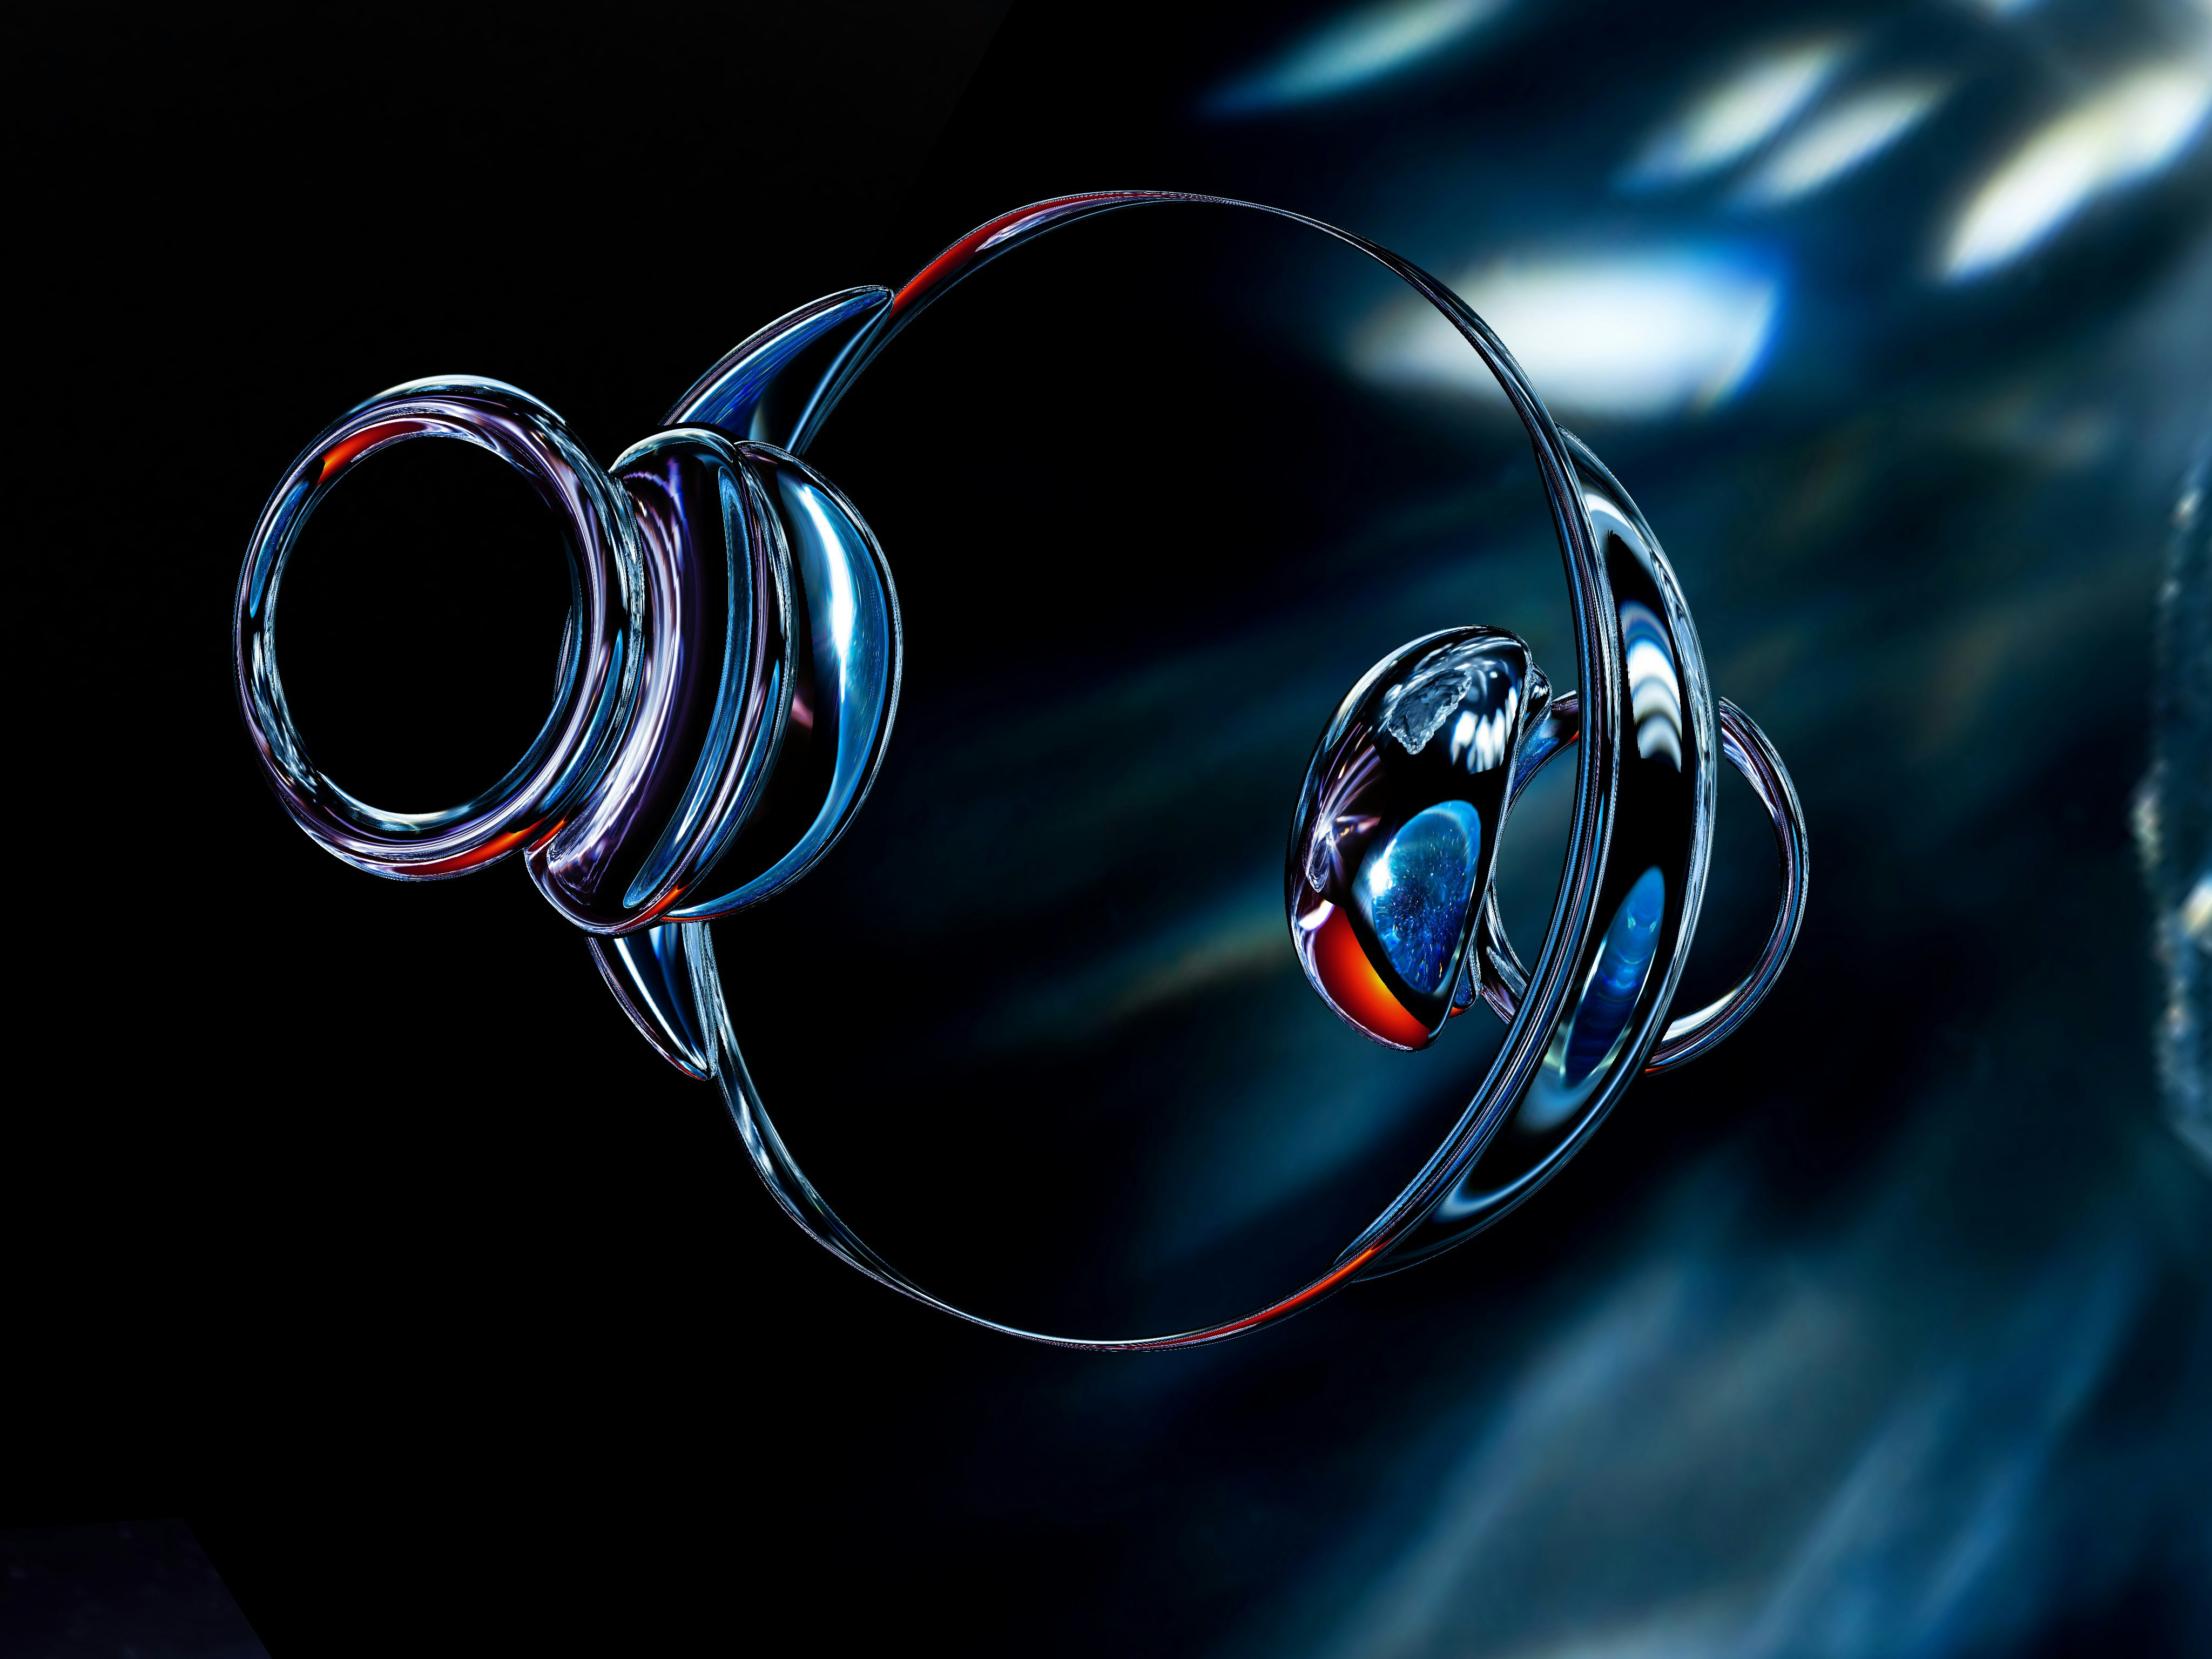
\includegraphics[width=1\paperwidth,height=0.5\paperheight]{img/luis-vasconcelos-wxj729MaPRY-unsplash.jpg}};%height=0.5\paperheight %% https://unsplash.com/de/fotos/blaues-und-rotes-licht-digitales-hintergrundbild-wxj729MaPRY
 %\node[opacity=1,inner sep=0pt] at (0.37\paperwidth,0.4\paperheight){
\includegraphics[scale=0.5]{img/gau-1.pdf}};
 \node at (0.25\paperwidth, 0.45\paperheight) {
\includegraphics[scale=0.65]{img/gau-1.pdf}};
\end{tikzpicture}}
}

\makeatletter                   
\def\printauthor{%                  
    {\large \@author}}          
\makeatother

\begin{titlepage}
\BgThispage
\newgeometry{left=00.5cm,right=6cm,bottom=3cm}
\vspace*{0.25\textheight}
\noindent
\hspace{0.5cm}
\textcolor{white}{\Huge\textbf{\textsf{\maniflow}}} %the titles
\vspace*{0.25cm}\par
\hspace{-0.055cm}
\textcolor{white}{\large\textbf{\textsf{A Python library for geometric processing}}}
\hspace{-20pt}
\vspace*{10cm}\par
\noindent
\hspace*{0.4\paperwidth}
\begin{minipage}{0.4\linewidth} %author info
    \begin{flushright}
        \printauthor
    \end{flushright}
\end{minipage} \hspace{15pt}
%
\begin{minipage}{0.9\linewidth} %the ornament
    \hspace{-0.5cm}
    \begin{tikzpicture}
        \node[rotate=90] at (0,0) {\pgfornament[width=3cm, color=titlepagecolor]{86}};
    \end{tikzpicture}
\end{minipage} \hspace{-10pt}
%
\end{titlepage}
\pagenumbering{arabic}
\pagenumbering{gobble}
\begin{abstract}
    The purpose of this library is to provide tools for the study of the most beautiful discipline of mathematics: geometry and geometric analysis. In doing so, we restrict ourselves to 2-manifolds. For a mathematician, this may initially seem like a major restriction. However, it allows us, in a relatively simple way, to represent 2-manifolds as ''meshes`` and to develop powerful tools to study them. 
    
    The abstraction hardly needs to be restricted at all, because the proposed calculus for meshes makes it possible to develop new geometries with comparatively little effort. Properties of these meshes can then be examined using \maniflow. For example, we provide tools to break down meshes into their connected components. You can also use \maniflow{} to determine the orientability of a mesh. It is also possible to run a geometric flow, such as the mean curvature flow, on a mesh. This means that \maniflow{} can also be used to examine meshes with regard to curvature (Gaussian curvature, mean curvature).
    
    \maniflow{} also provides the option of creating images of the meshes. This makes it possible, for example, to create animations of geometric flows etc.
\end{abstract}
\tableofcontents
\listoffigures
\vfill
\hrule\vspace*{0.2cm}
\noindent\footnotesize{\maniflow{} was developed as part of the course M.Mat.0731 ''Advanced practical course in scientific computing`` at Georg-August University Göttingen.

The image on the frontpage is taken from \href{https://unsplash.com/de/fotos/blaues-und-rotes-licht-digitales-hintergrundbild-wxj729MaPRY}{\url{https://unsplash.com/de/fotos/blaues-und-rotes-licht-digitales-hintergrundbild-wxj729MaPRY}}
\restoregeometry
\normalsize
\pagenumbering{arabic}
\newpage
\section*{Getting started}
\addcontentsline{toc}{section}{Getting started}
\epigraph{\footnotesize{``Be patient, for the world is broad and wide.``}}{\footnotesize{-- \textsc{E. A. Abbott}, Flatland: A Romance of Many Dimensions }}
The code of \maniflow{} was originally published on
\begin{center}
    \qrcode{https://gitlab.gwdg.de/yangshan.xiang/scientific-computing}\\
    \vspace*{0.5cm}
    \href{https://gitlab.gwdg.de/yangshan.xiang/scientific-computing}{\url{https://gitlab.gwdg.de/yangshan.xiang/scientific-computing}}
\end{center}
To install the libary, simply use
\begin{center}
    \boxedcode{\texttt{pip install dist/maniflow-1.0-py2.py3-none-any.whl}}
\end{center}
To build the wheel file of the library, use
\begin{center}
    \boxedcode{\texttt{python setup.py bdist\_wheel --universal}}
\end{center}
\paragraph{Dependencies.} The installation and usage of \maniflow{} requires the following packages to be installed: \href{https://numpy.org/}{\texttt{numpy}}, \href{https://pillow.readthedocs.io/en/stable/}{\texttt{pillow}}
\paragraph{Optional dependencies.} When using \texttt{maniflow.render.SVGPainterRenderer}, one requires the installation of \href{https://pypi.org/project/drawsvg/}{\texttt{drawsvg}}.
\section{Introduction}
First, we will look at the basic mathematical concepts that ultimately underpin the whole theory. So let's start with so-called meshes and look at some examples and how these mathematical concepts can be implemented in code using \maniflow{}.
\begin{defi}[Mesh]
    Let $V$ be a vector space  over $\R$ of dimension $n$. Let $\mathcal{V}_M\subset V$ be a set of points in $V$. We further let $\mathcal{F}_M\subset\mathcal{V}_M^3$. The pair $M = (\mathcal{V}_M, \mathcal{F}_M)$ is then called mesh. The elements of $\mathcal{V}_M$ are called points of $M$ and the elements of $\mathcal{F}_M$ are the faces of the mesh $M$.
\end{defi}
For a mesh $M = (\mathcal{V}_M, \mathcal{F}_M)$ we will often denote $V_M = \vert\mathcal{V}_M\vert$ and $F_M = \vert\mathcal{F}_M\vert$.
\paragraph{Remark.} Meshes $M$ can be considered as $2$-dimensional simplicial complexes. Thus for $2$-dimensional manifolds $\Tilde{M}\subset V$ we may find a \textit{triangulation} simplicial complex $K$ of $\Tilde{M}$. The corresponding mesh will be called \textit{triangulation} mesh of the manifold $\Tilde{M}$.
\begin{ex}[Tetrahedron]\label{ex:tetra} Let 
\begin{align*}
    \mathcal{V} = \left\{\left(\sqrt{\frac89},0,-\frac13\right),\left(-\sqrt{\frac29},\sqrt{\frac23},-\frac13\right),\left(-\sqrt{\frac29},-\sqrt{\frac23},-\frac13\right), \left(0,0,1\right)\right\}\subset\R^3
\end{align*}
and $\mathcal{F} = \{f\in2^{\mathcal{V}}:\vert f\vert = 3\}$. The mesh $T = (\mathcal{V},\mathcal{F})$ is the tetrahedron, which is displayed in figure \ref{fig:tetra}.
    \begin{figure}[h]
        \centering
        \includesvg[scale=0.6]{img/tetrahedron.svg}
        \caption{Tetrahedron}
        \label{fig:tetra}
    \end{figure}
This can be implemented using \texttt{maniflow} by using the \texttt{Mesh} class:
\begin{lstlisting}
import numpy as np
import itertools
from maniflow.mesh import Mesh, Face

# computing the four vertices of the tetrahedron
v1 = np.array([np.sqrt(8/9), 0, -1/3])
v2 = np.array([-np.sqrt(2/9), np.sqrt(2/3), -1/3])
v3 = np.array([-np.sqrt(2/9), -np.sqrt(2/3), -1/3])
v4 = np.array([0, 0, 1])

tetra = Mesh()
# setting the vertices as the vertices of the new mesh object
tetra.vertices = [v1, v2, v3, v4]
# now we compute the subsets of all the vertices consiting of three vertices
subsets = set(itertools.combinations(list(range(tetra.v)), 3))
# the faces are then set as the faces of tetra
tetra.faces = [Face(tetra, *list(i)) for i in subsets]
\end{lstlisting}
This way, we obtain the \texttt{Mesh} object \texttt{tetra} which represents a tetrahedron.
\end{ex}
\subsection{Reading and writing \texttt{.obj} files}\label{sec:objfiles}
The repeated computation of meshes can require a lot of computing capacity under certain circumstances. It can also be difficult to programme complicated geometries line by line in the code. To avoid these difficulties, \maniflow{} supports the \texttt{.obj} file format.
This makes it possible to export meshes for further editing in other programmes (e.g. \href{https://www.blender.org/}{Blender} or similar) or to display them\footnote{if you do not want to use the internal renderer of \maniflow{}}.
You can also use third-party software to create complicated geometries relatively easily and import them into \maniflow{}.
Interaction with .obj files is made possible by the maniflow.mesh.obj.OBJFile class.
\paragraph{Caution:} \texttt{maniflow.mesh.obj.OBJFile} currently disregards any normal vectors, texture coordinates, line elements etc. defined in the \texttt{.obj} file.
Only the coordinates of the vertices are taken into account and for the faces only the indices of the vertices that make them up are taken into consideration.
\begin{ex}
    Consider the \texttt{Mesh} object \texttt{tetra} from example \ref{ex:tetra}. To store this mesh in a \texttt{.obj} file, we may use
    \begin{lstlisting}
from maniflow.mesh.obj import OBJFile

OBJFile.write(tetra, "examples/tetrahedron.obj")
    \end{lstlisting}
    This code produces the file \url{examples/tetrahedron.obj}. In order to load a mesh into \maniflow{}, simply use
    \begin{lstlisting}
mesh = OBJFile.read("examples/tetrahedron.obj")
    \end{lstlisting}
\end{ex}
\subsection{\texttt{maniflow.mesh.utils.VertexFunction} -- Creating meshes from parameterisations}
The way we created a mesh of a tetrahedron in the previous example is very static and absolutely not suitable if you want to study more complicated geometries. \maniflow{}, however, provides the option of creating meshes quite easily using parameterisations. For this purpose, \maniflow{} provides the wrapper \texttt{maniflow.mesh.utils.VertexFunction}, which executes a given function on all vertices of the mesh and has the resulting mesh as output.
\begin{ex}
    For the following example, we assume that we have a \texttt{Mesh}-object \code{mesh} and we want to shift this mesh by the vector $\begin{pmatrix}1 & 2 & 3\end{pmatrix}^{\intercal}\in\R^3$. For this we make use of a \texttt{VertexFunction}:
    \begin{lstlisting}
# importing the wrapper from maniflow.mesh.utils
from maniflow.mesh.utils import VertexFunction

# implementing the VertexFuntion 'shift'
@VertexFuntion
def shift(vertex):
    return vertex + np.array([1, 2, 3])


# applying 'shift' to 'mesh'
shifted = shift(mesh)
    \end{lstlisting}
    The resulting \texttt{Mesh}, \code{shifted}, is \code{mesh} shifted by the vector $\begin{pmatrix}1 & 2 & 3\end{pmatrix}^{\intercal}\in\R^3$.
\end{ex}
Another application of this would be the creation of meshes from parameterisations $\psi\colon \R^2\supset D\to\R^3$. Oftentimes, the domain $D$ is a cartesian product of two intervals, so $D = I_1\times I_2$.\footnote{Or to be more precise, \maniflow{} makes it easy to create meshes from parametrisations, where the domain $D$ is homoeomorphic to a square.} For this, \maniflow{} provides the class \texttt{maniflow.mesh.parameterized.Grid}.
\begin{ex}[Moebius strip]\label{ex:moebius_creation}
We now turn to an example where we want to create a triangulation of a moebius strip. To this end, we will use the parametrisation
\begin{align*}
    \psi\colon [0, 2\pi]\times [-1,1]\to\R^3,\ (u,v)\mapsto\begin{pmatrix}
        \left(1+\frac{v}{2}\cos{\frac{u}{2}}\right)\cos{u}\\
        \left(1+\frac{v}{2}\cos{\frac{u}{2}}\right)\sin{u}\\
        \frac{v}{2}\sin{\frac{u}{2}}
    \end{pmatrix}.
\end{align*}
In order to discretise the set $[0,2\pi]\times[-1,1]$, we make use of \texttt{maniflow.mesh.parametrized.Grid} in order to create a high resolution lattice. Then we can implement a \texttt{VertexFunction} to capture the parametrisation $\psi$ in code and apply it to our lattice.
\begin{lstlisting}
from maniflow.mesh.parameterized import Grid
from maniflow.mesh.utils import VertexFunction


# implementing the parametrisation 1:1 in code as a VertexFunction
@VertexFunction
def moebius(vertex):
    x = vertex[0]
    y = vertex[1]
    x0 = np.cos(x) * (1 + (y / 2) * np.cos(x / 2))
    x1 = np.sin(x) * (1 + (y / 2) * np.cos(x / 2))
    x2 = (y / 2) * np.sin(x / 2)
    return np.array([x0, x1, x2])


u = Grid((0, 2 * np.pi), (-1, 1), 30, 10)  # create a high resolution grid
moebiusMesh = moebius(u)  # mapping the vertices from the grid according to the parametrisation
coincidingVertices(moebiusMesh) # remove the redundant vertices at the joint after making the moebius band
\end{lstlisting}
With this we obtain the \texttt{Mesh}-object \code{moebiusMesh}. Using \texttt{maniflow.mesh.obj.OBJFile}, we can write this mesh to memory as a \texttt{.obj} file, see section \ref{sec:objfiles}
\begin{lstlisting}
from maniflow.mesh.obj import OBJFile

OBJFile.write(moebiusMesh, "examples/moebius.obj")
\end{lstlisting}
Unsurprisingly, one can then load this file into \href{https://www.blender.org/}{Blender} and create pictures of it etc.\footnote{\maniflow{} comes with its own simple renderer. But if you want to do more elaborated computer graphics, you might consider using some other software to render images.} Figure \ref{fig:moubius_blender} shows a screenshot taken from Blender with the \texttt{.obj} file from \href{https://gitlab.gwdg.de/yangshan.xiang/scientific-computing/-/blob/82c42c864b3e46303b208b78720b8109116c78da/examples/moebius.obj}{\url{examples/moebius.obj}}.
\end{ex}
\begin{figure}[t]
    \centering
    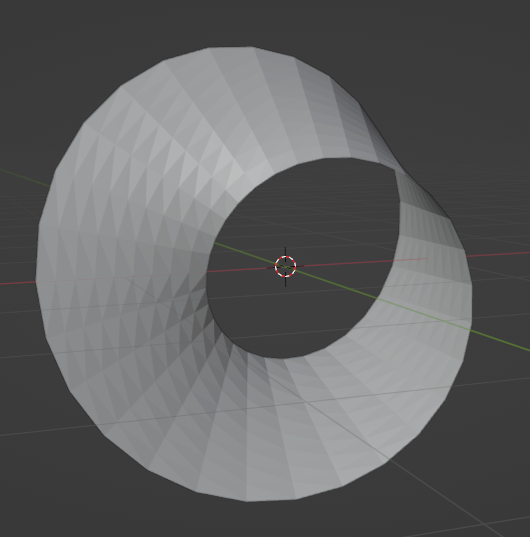
\includegraphics[scale=0.35]{img/moebius_2023-05-23.png}
    \caption{Screenshot of \href{https://www.blender.org/}{Blender} with a moebius strip made with \maniflow{}}
    \label{fig:moubius_blender}
\end{figure}
\newpage
\section{The face graph of a mesh}
\begin{defi}[Undirected Graph]
    Let $\V_G$ be a set and $\E_G\subset\{e\in2^{\V_G}: |e|=2\}$ be a set of unordered pairs of elements from $\V_G$. The pair $G = (\V_G, \E_G)$ is then called undirected Graph. The elements from $\V_G$ are called vertices of $G$ and the elements from $\E_G$ are called edges of $G$.
\end{defi}
For a Graph $G=(\V_G,\E_G)$ we write
\begin{align*}
    \vcenter{\hbox{\begin{tikzpicture}
    \node (A) at (0,0) {$x$};
    \node (B) at (1,0) {$y$};
    \draw[-] (A) -- (B);\end{tikzpicture}}}
\end{align*}
if $\{x,y\}\in\E_G$. If we take all edges and points together in this way, we get the picture
of a graph with undirected edges.
\begin{ex}
    \begin{equation}\label{eq:sample_g}
    G\colon\left(\vcenter{\hbox{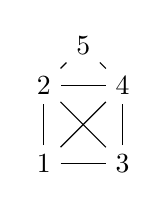
\begin{tikzpicture}[scale=0.5]
    \node (1) at (-1,-1) {$1$};
    \node (2) at (-1,1) {$2$};
    \node (3) at (1,-1) {$3$};
    \node (4) at (1,1) {$4$};
    \node (5) at (0,2) {$5$};
    \draw[-] (1) -- (2);
    \draw[-] (2) -- (3);
    \draw[-] (3) -- (4);
    \draw[-] (4) -- (2);
    \draw[-] (2) -- (5);
    \draw[-] (5) -- (4);
    \draw[-] (4) -- (1);
    \draw[-] (1) -- (3);
\end{tikzpicture}}}\right),\qquad H\colon\left(\vcenter{\hbox{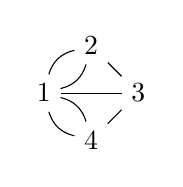
\begin{tikzpicture}[scale=0.6]
\node (1) at (-1, 0) {$1$};
\node (2) at (0, 1) {$2$};
\node (3) at (1,0) {$3$};
\node (4) at (0,-1) {$4$};
\draw[-] (1) -- (3);
\path [-] (1) edge[bend right=-30](2); 
\path [-] (1) edge[bend right=30](2); 
\path [-] (1) edge[bend right=-30](4); 
\path [-] (1) edge[bend right=30](4);
\draw[-] (3) -- (2);
\draw[-] (4) -- (3);
\end{tikzpicture}}}\right)
\end{equation}
\end{ex}
\begin{defi}[Face Graph]
    Let $M = (\mathcal{V}_M, \mathcal{F}_M)$ be a mesh and
    \begin{align*}
        \mathcal{E} = \left\{(f_1,f_2)\in\mathcal{F}_G^2: \vert f_1\cap f_2\vert =2\right\}
    \end{align*}
    The face graph of $M$ is the graph $(\mathcal{F}_M,\mathcal{E})$.
\end{defi}
\begin{ex} The face graph of the tetrahedron is given by
    \begin{equation}\label{eq:sample_g1}
    G\colon\left(\vcenter{\hbox{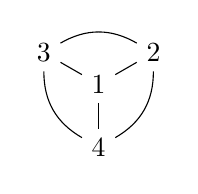
\begin{tikzpicture}[scale=0.8]
    \node (1) at (0,0) {$1$};
    \node (2) at (0.87,0.5) {$2$};
    \node (3) at (-0.87,0.5) {$3$};
    \node (4) at (0,-1) {$4$};
    \draw[-] (1) -- (2);
    \draw[-] (1) -- (3);
    \draw[-] (1) -- (4);
    \path[-] (2) edge[bend right=30] (3);
    \path[-] (3) edge[bend right=30] (4);
    \path[-] (4) edge[bend right=30] (2);
\end{tikzpicture}}}\right)
\end{equation}
\end{ex}
The face graph of a given mesh can be constructed by algorithm \ref{alg:facegraph}.
\begin{algorithm}
    \SetKwInOut{Input}{Input}
    \SetKwInOut{Output}{Output}

    \Input{A mesh $M = (\mathcal{V}_M, \mathcal{F}_M=\{f_1,f_2,f_3\ldots\})$}
    \Output{The adjacency matrix of the face graph of the mesh $M$}
    \caption{Construction of the face graph of a given mesh}
    \label{alg:facegraph}
    $G := 0\in\R^{F_M\times F_M}$\;
    \For{$i=1$ \KwTo $F_M$}
    {
        $neighbors := 0$\;
        \For{$j=1$ \KwTo $F_M$}
        {
            \If{$neighbors = 3$}{
            \textbf{break}\;
            }
            \If{$\vert f_i\cap f_j\vert = 2$ \normalfont{\textbf{and}} $i\neq j$}{
            $G_{ij} \leftarrow 1$\;
            $neighbors \leftarrow neighbors + 1$\;
            }
        }
    }
    \Return{$G$}
\end{algorithm}
Since this algorithm loops over the faces of the mesh in a nested way, the complexity of it lies in $O(F_M^2)$. As this runtime complexity has the consequence of the algorithm being very slow at execution for somewhat large meshes, the face graph is computed dynamically by \texttt{maniflow.mesh.Mesh.faceGraph}.
\subsection{A first application: \texttt{maniflow.mesh.utils.connectedComponents}}
The method \texttt{maniflow.mesh.utils.connectedComponents} decomposes the given mesh into its connected components. Now that we have an algorithm with which to compute the face graph, the connected components of a mesh can now be identified as the connected components of the face graph. These can be determined via the breadth-first traversal of the face graph. 
\begin{algorithm}
    \SetKwInOut{Input}{Input}
    \SetKwInOut{Output}{Output}

    \Input{A mesh $M = (\mathcal{V}_M, \mathcal{F}_M=\{f_1,f_2,f_3\ldots\})$}
    \Output{The connected components of the mesh $M$}
    \caption{Construction of the face graph of a given mesh}
    \label{alg:components}
    Compute the adjacency matrix $G$ using \ref{alg:facegraph}\;
    $start := 1$\;
    $n := 1$\;
    \While{$\mathcal{F}_M\neq\emptyset$}{
        Compute a breadth first traversal sequence $T_n \leftarrow \{f_{start}, f_b,f_c,\ldots\}\subseteq\mathcal{F}_M$\;
        $n \leftarrow n+1$\;
        $\mathcal{F}_M\leftarrow \mathcal{F}_M\setminus T_n$\;
        Set $1< start\leq F_M$ such that $f_{start}\in\mathcal{F}_M$\;
    }
    
    \Return{$T_1$, $T_2$, $\ldots$}
\end{algorithm}
\paragraph{Runtime analysis.} Algorithm \ref{alg:facegraph} has a runtime complexity which lies in $O(F_M^2)$. The breadth-first traversal on the face graph has a runtime\footnote{Since on a graph with the number of vertices being $V$ and the number of edges being $E$ the breadth first search has a complexity of $O(E + V)$. As every face has at most three neighbors we obtain the given runtime complexity.} complexity of $O(F_M + 3\cdot F_M) = O(F_M)$. The computation of $\mathcal{F}_M\setminus T_n$ has also quadratic complexity $O(\vert\mathcal{F}_M\vert^2)$. Thus the overall complexity of algorithm \ref{alg:components} lies in $O(F_G^2)$.
\begin{ex}
    In this example we analyse the connected components of the teapot from \texttt{examples/teapot.obj}. The teapot is displayed in figure \ref{fig:teapot}.
    \begin{figure}[h]
        \centering
        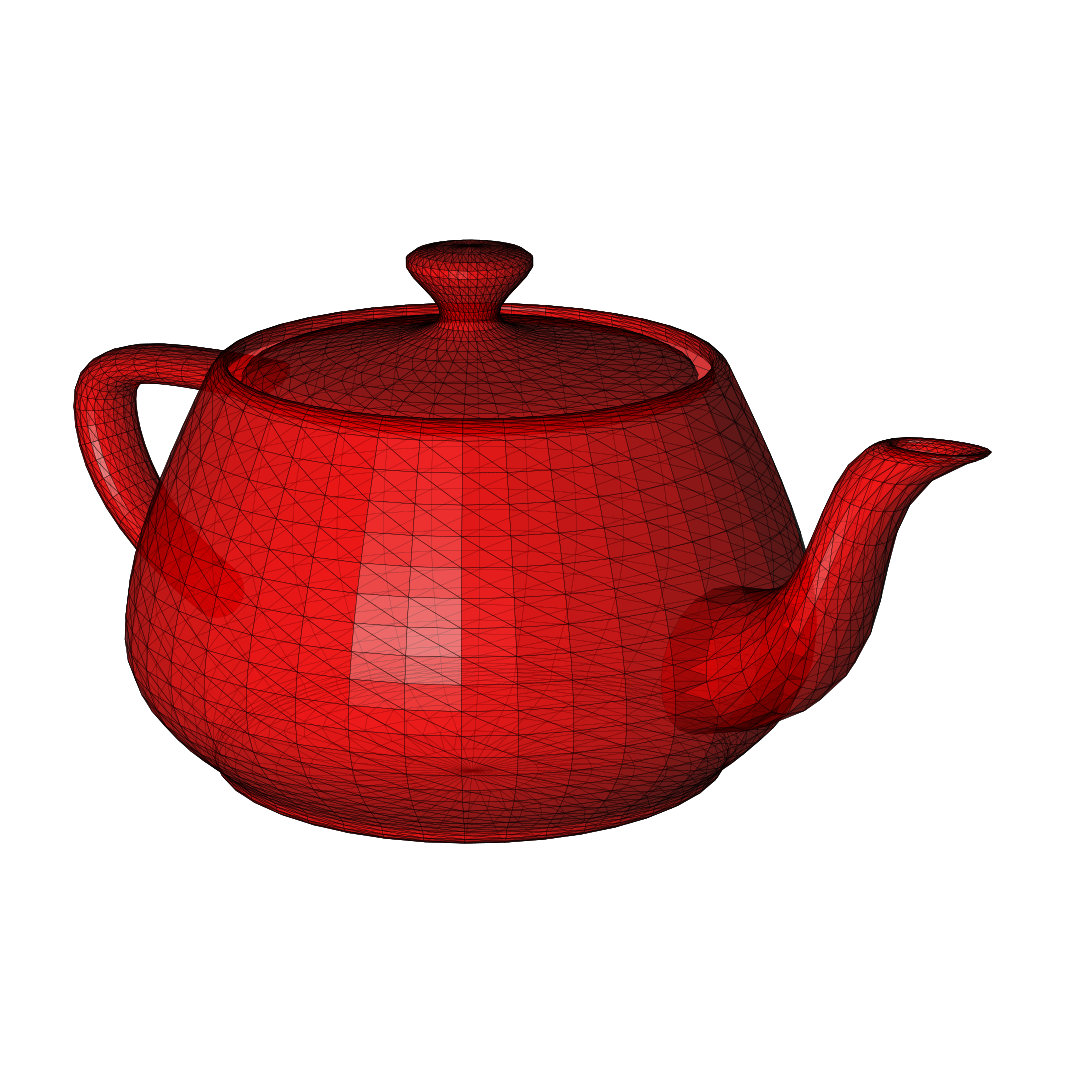
\includegraphics[scale=0.15]{img/teapot.png}
        \caption{The teapot from \texttt{examples/teapot.obj}}
        \label{fig:teapot}
    \end{figure}
    \newline\noindent The connected components can be computed using the following code
    \begin{lstlisting}
from maniflow.mesh import Mesh
from maniflow.mesh.obj import OBJFile
from maniflow.mesh.utils import connectedComponents, coincidingVertices

teapot = OBJFile.read("examples/teapot.obj")  # reading the mesh from memory
coincidingVertices(teapot)  # identifying and collapsing coinciding vertices

# now we compute the connected components
components = connectedComponents(teapot)

# we can now reconstruct meshes from these lists of faces and write them to .obj files
for i, component_list in enumerate(components):
    component = Mesh.fromFaceList(teapot, *component_list)
    OBJFile.write(component, "teapot" + str(i + 1) + ".obj")
    \end{lstlisting}
    The resulting components are shown in figure \ref{fig:teapotcomps}.
    \begin{figure}[ht]
    \centering
    \subfloat[The lid of the teapot]{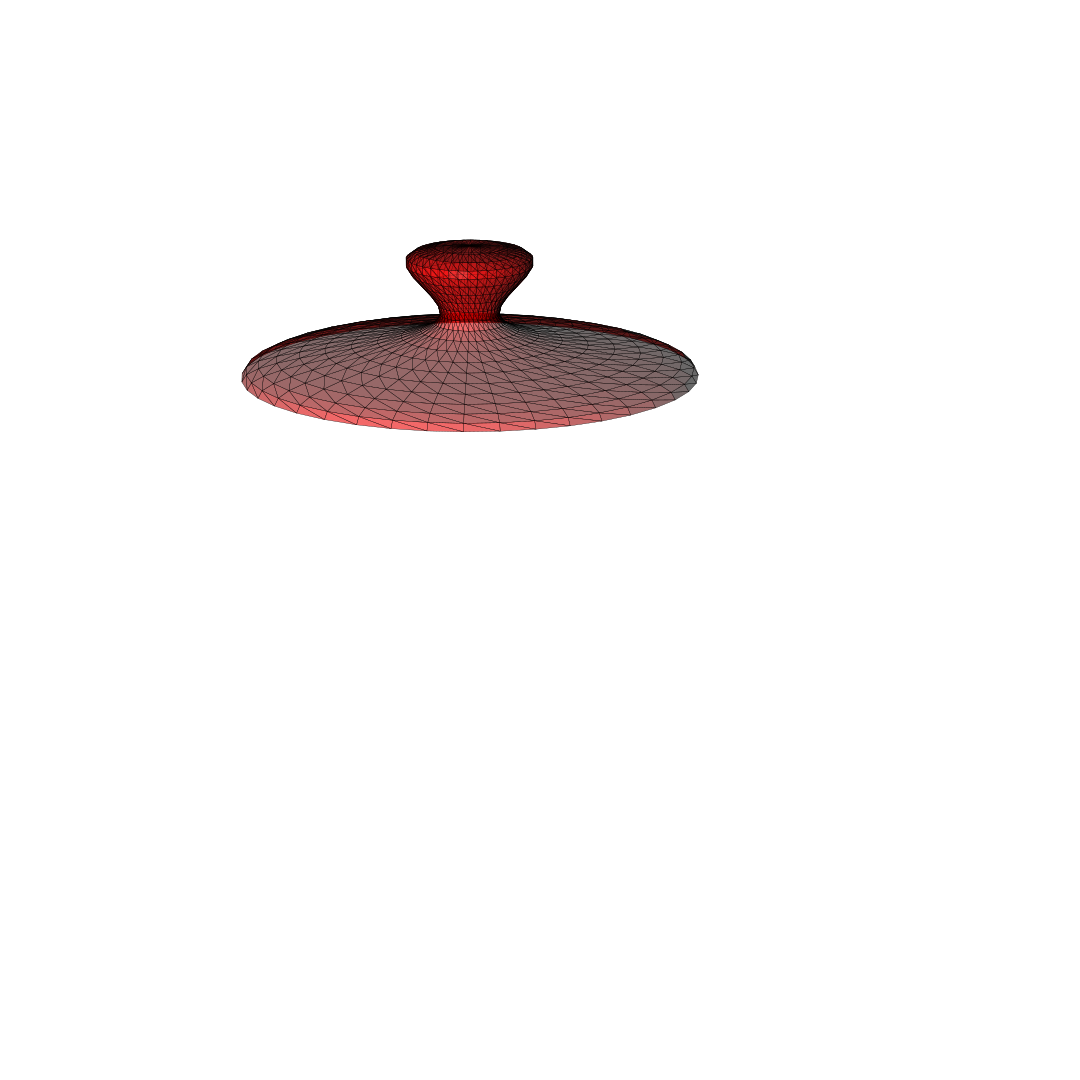
\includegraphics[width=0.4\textwidth]{img/teapot1.png}}\hfil
    \subfloat[The handle of the teapot]{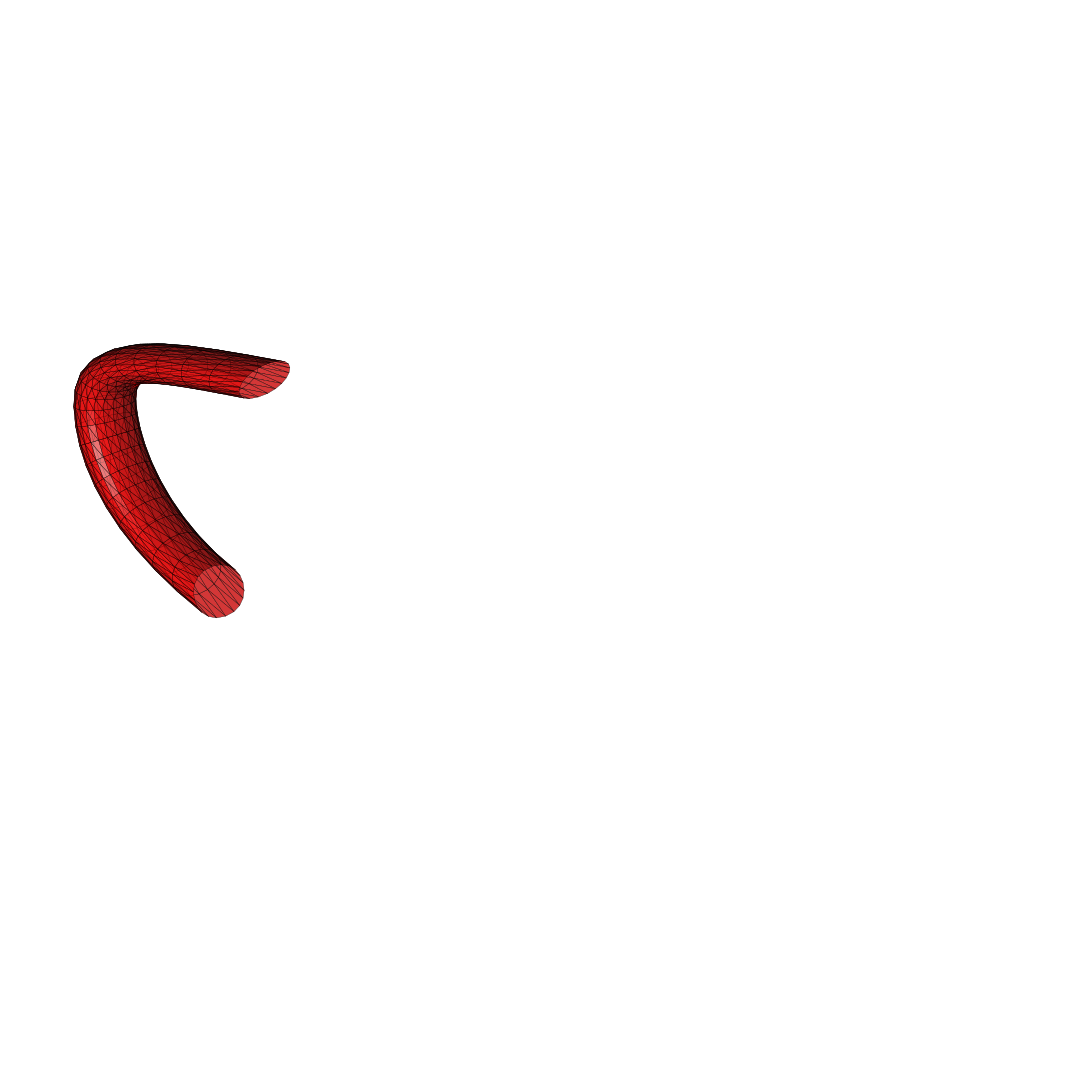
\includegraphics[width=0.4\textwidth]{img/teapot2.png}}\hfil\\
    \subfloat[The body of the teapot]{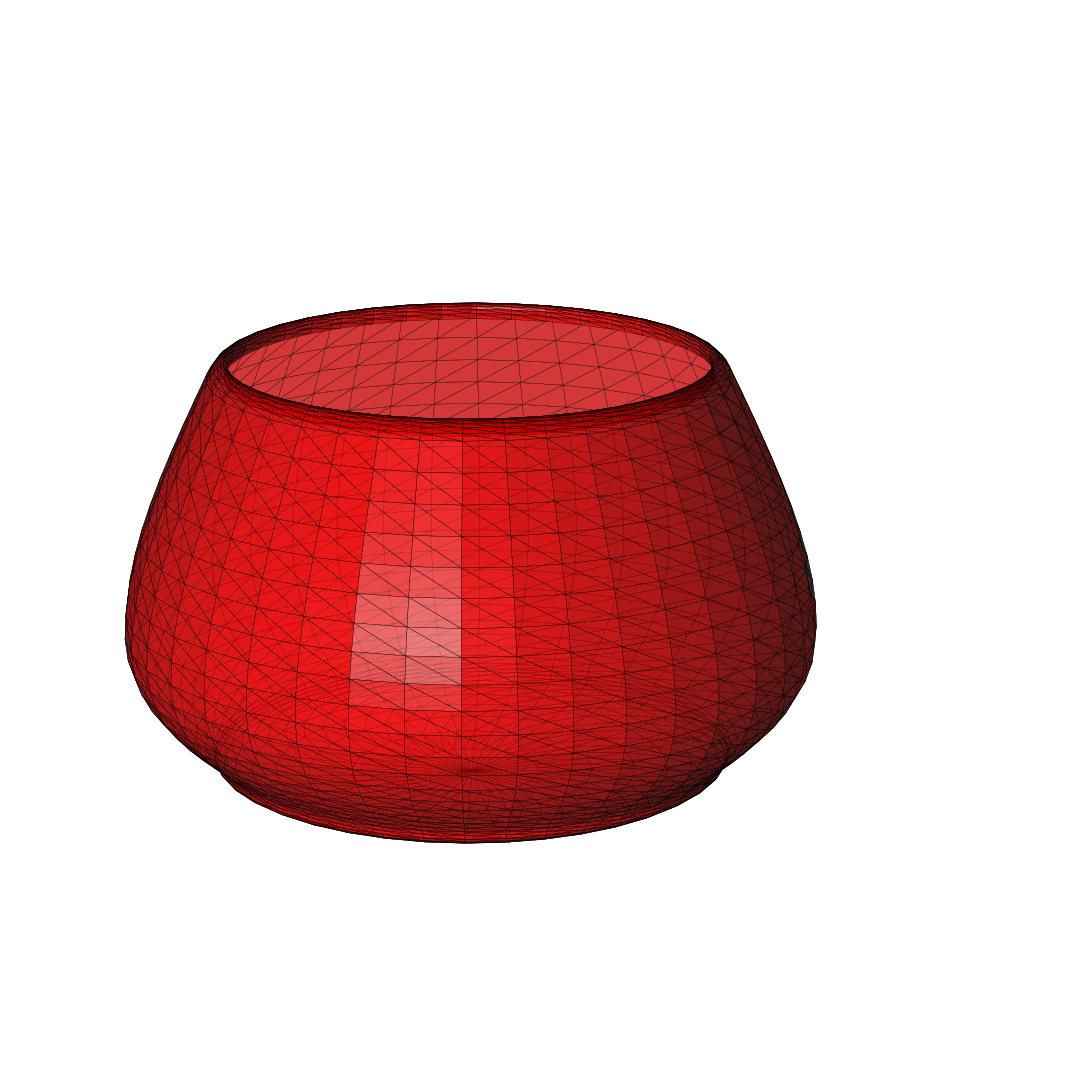
\includegraphics[width=0.4\textwidth]{img/teapot3.png}}\hfil
    \subfloat[The spout of the teapot]{
\includegraphics[width=0.4\textwidth]{img/teapot4.png}}\hfil
    \caption{The connected components of the teapot}
    \label{fig:teapotcomps}
\end{figure}
\end{ex}
\subsection{Another application: checking orientability of a \texttt{Mesh}}
Orientability is an important property of manifolds in geometry. For example, the area can only be meaningfully defined for orientable 2-manifolds. For 2-manifolds embedded in $\R^3$, orientability is equivalent to the existence of a continuous unit-normal vector field on the manifold. Similarly, we can extend the notion of orientability to meshes. If we consider a face spanned by the vertices $v_1,\ v_2$ and $v_3$, the normal vector is, for example given by\footnote{Note that $n$ does not necessarily have length $1$. But one may always obtain a unit normal vector by rescaling}
\begin{align*}
    n = (v_1 - v_2)\times (v_1 - v_3).
\end{align*}
Hence, the orientation or direction of $n$ is dependent upon the enumeration of the vertices that define the face. A priori it is not clear that two neighboring faces really do have ``compatible'' enumerations of their vertices. So it may happen that two neighboring faces have normal vectors that point in ``opposite'' directions.\footnote{An appeal to the reader's intuition. You have to be careful with these notions.}
\begin{defi}[Orientation of faces]
    Let $f = (v_1, v_2, v_3)$ be a face defined by the vertices $v_i$ for $1\leq i\leq 3$. Let $f'$ be another face that is defined by the vertices $v_1,\ v_2$ and $v_{\ast}$. We say that two faces have the same orientation, if there is a cyclic permutation $\sigma\in S_3$ such that
    \begin{align*}
        (f_1, f_2) = (f'_{\sigma(2)},f'_{\sigma(1)}).
    \end{align*}
    Where $f_i$ and $f'_i$ denote the $i$-th vertex in the faces $f$ and $f'$ respectively.
\end{defi}
In other words, two faces have the same orientation if they share an edge and that edge is traversed in opposite directions, when listing the vertices of the faces, see figure \ref{fig:orientation}.
\begin{ex}
    Consider the faces $f = (1, 2, 3)$ and $f' = (2, 3, 4)$. Then $f$ and $f'$ share the edge made up of the vertices $2$ and $3$. But both of them traverse this edge in the same direction $(2,3)$. On the other hand, if we changed the enumeration of $f'$ to $(3, 2, 4)$, the faces would have matching orientation. This is exactly the situation depicted in figure \ref{fig:orientation}.
\end{ex}
\begin{figure}[ht]
    \centering
    \subfloat[Non compatible orientation]{
    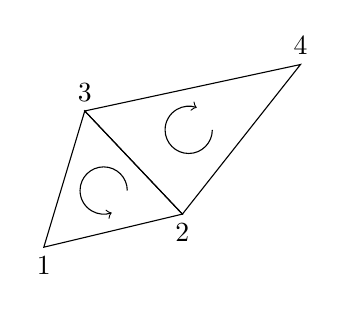
\begin{tikzpicture}
        \draw[]{} (-1.1, -1.13) -- (0.66, -0.71) node[below]{$2$} -- (-0.58, 0.6) node[above]{$3$} -- cycle node[below]{$1$};
        \draw[]{} (0.66, -0.71) -- (-0.58, 0.6) -- (2.16, 1.19) node[above]{$4$} -- cycle;
        \draw[->] (-0.04,-0.41) arc[radius=0.3cm,start angle=0,delta angle=290];
        \draw[->] (1.04,0.36) arc[radius=0.3cm,start angle=0,delta angle=-290];
    \end{tikzpicture}
    }
    \subfloat[Compatible orientation]{
    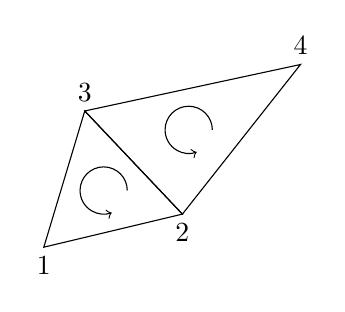
\begin{tikzpicture}
        \draw[]{} (-1.1, -1.13) -- (0.66, -0.71) node[below]{$2$} -- (-0.58, 0.6) node[above]{$3$} -- cycle node[below]{$1$};
        \draw[]{} (0.66, -0.71) -- (-0.58, 0.6) -- (2.16, 1.19) node[above]{$4$} -- cycle;
        \draw[->] (-0.04,-0.41) arc[radius=0.3cm,start angle=0,delta angle=290];
        \draw[->] (1.04,0.36) arc[radius=0.3cm,start angle=0,delta angle=290];
    \end{tikzpicture}
    }
    \caption{Two triangles with compatible and non compatible orientations}
    \label{fig:orientation}
\end{figure}
In order to determine whether a given mesh is orientable or not, we can sort of ``push'' an orientation to the mesh by traversing each of the faces in breadth-first traversal and adjusting the orientations / enumerations of vertices of each of the neighboring faces for the currently traversed face.\footnote{Of course we have to remember the faces we already considered while traversing the mesh in order to avoid faces being re-oriented twice.}
\begin{algorithm}
    \SetKwInOut{Input}{Input}
    \SetKwInOut{Output}{Output}

    \Input{A mesh $M = (\mathcal{V}_M, \mathcal{F}_M=\{f_1,f_2,f_3\ldots\})$}
    \caption{Pushing an orientation to a mesh}
    \label{alg:pushorientation}
    Store the connected components of $M$ in $\mathcal{C}$ (see algorithm \ref{alg:components})\;
    \For{$c\in\mathcal{C}$}{
    $visited := \emptyset$\;
    \For{$f\in c$}{
    \If{$f\notin visited$}{
    Store neighbouring faces to $f$ in $neighbours$\;
    \For{$f_n\in neighbours$}{
    \If{$f$ and $f_n$ do not have compatible orientations}{
    reverse the enumeration of vertices in $f_n$\;
    }
    }
    $visited \leftarrow visited \cup \{ f\}$\;
    }
    }
    }
\end{algorithm}
This is what algorithm \ref{alg:pushorientation} does. The method \texttt{maniflow.mesh.utils.pushOrientation} implements this algorithm in \maniflow{}.
Finally, to check whether a mesh is orientable or not, we only need to iterate over all surfaces in the mesh and ask whether all neighbours have a compatible orientation. This is implemented as the method \texttt{maniflow.mesh.utils.isOrientable}.
\paragraph{Runtime analysis.}  Algorithm \ref{alg:pushorientation} has a complexity of $O(F_M^2)$. % TODO: more details?
\begin{ex}[Orientability of the Moebius strip]
    Consider the \texttt{Mesh} object \texttt{moebiusMesh} from example \ref{ex:moebius_creation}. To determine whether this mesh is orientable or not, use
    \begin{lstlisting}
from maniflow.mesh.utils import isOrientable

print(isOrientable(moebiusMesh))
    \end{lstlisting}
    As expected, the output will be \texttt{False} as the Moebius strip is not orientable.
\end{ex}
\noindent Another example that is less trivial than the Moebius strip is documented in the file \href{https://gitlab.gwdg.de/yangshan.xiang/scientific-computing/-/blob/28846b92bf3f99fa84b650267886782c43791715/examples/roman_surface.ipynb}{\url{examples/roman\_surface.ipynb}} where the so-called Roman surface is discussed.

\documentclass{article}
\usepackage[utf8]{inputenc}
\usepackage{amsmath}
\usepackage{amsfonts}
\usepackage{graphicx}
\usepackage{amssymb}
\usepackage{amsthm}
\usepackage{float}
\usepackage{tikz}
\usepackage{mlmodern}
\usepackage{subfig}
\usepackage[T1]{fontenc}
\usepackage[left=2.5cm,right=2.5cm]{geometry}
\usepackage[linesnumbered,ruled]{algorithm2e}

\usepackage{svg}

\usepackage{listings}
\newcommand{\code}[1]{\texttt{#1}} % inline code setting
\renewcommand{\lstlistingname}{Code}

\definecolor{codebg}{RGB}{230,230,230}
\lstset {
    breakatwhitespace=false,         % sets if automatic breaks should only happen at whitespace
    breaklines=true,                 % sets automatic line breaking
    captionpos=b,                    % sets the caption-position to bottom
    tabsize=4,
    %showstringspaces=false,
    numbers=left,                    % where to put the line-numbers; possible values are (none, left, right)
    numbersep=2pt,                   % how far the line-numbers are from the code
    numberstyle=\tiny, % the style that is used for the line-numbers
    %upquote=true,
    backgroundcolor = \color{codebg},
    basicstyle=\small\ttfamily, % basic font setting
    emph={int,char,double,float,unsigned,void,bool},
    %emphstyle={\color{blue}},
    escapechar=\&,
    columns=fixed
}

\newtheorem{defi}{Definition}
\newtheorem{ex}{Example}
\newtheorem{prop}{Proposition}
\newtheorem{theorem}{Theorem}
\newtheorem{lemma}{Lemma}
\newtheorem{kor}{Corollary}

\newcommand{\N}{\mathbb{N}}

\newcommand{\R}{\mathbb{R}}
\newcommand{\V}{\mathcal{V}}
\newcommand{\E}{\mathcal{E}}

\title{\texttt{maniflow} -- a (partial) documentation}
\author{Felix Widmaier}
\date{}


\begin{document}
\maketitle
\section{Introduction}
\begin{defi}[Mesh]
    Let $V$ be a vector space  over $\R$ of dimension $n$. Let $\mathcal{V}_M\subset V$ be a set of points in $V$. We further let $\mathcal{F}_M\subset\mathcal{V}_M^3$. The pair $M = (\mathcal{V}_M, \mathcal{F}_M)$ is then called mesh. The elements of $\mathcal{V}_M$ are called points of $M$ and the elements of $\mathcal{F}_M$ are the faces of the mesh $M$.
\end{defi}
For a mesh $M = (\mathcal{V}_M, \mathcal{F}_M)$ we will often denote $V_M = \vert\mathcal{V}_M\vert$ and $F_M = \vert\mathcal{F}_M\vert$.
\paragraph{Remark.} Meshes $M$ can be considered as $2$-dimensional simplicial complexes. Thus for $2$-dimensional manifolds $\Tilde{M}\subset V$ we may find a \textit{triangulation} simplicial complex $K$ of $\Tilde{M}$. The corresponding mesh will be called \textit{triangulation} mesh of the manifold $\Tilde{M}$.
\begin{ex}[Tetrahedron] Let 
\begin{align*}
    \mathcal{V} = \left\{\left(\sqrt{\frac89},0,-\frac13\right),\left(-\sqrt{\frac29},\sqrt{\frac23},-\frac13\right),\left(-\sqrt{\frac29},-\sqrt{\frac23},-\frac13\right), \left(0,0,1\right)\right\}\subset\R^3
\end{align*}
and $\mathcal{F} = \{f\in2^{\mathcal{V}}:\vert f\vert = 3\}$. The mesh $T = (\mathcal{V},\mathcal{F})$ is the tetrahedron, which is displayed in figure \ref{fig:tetra}.
    \begin{figure}[h]
        \centering
        \includesvg[scale=0.6]{img/tetrahedron.svg}
        \caption{Tetrahedron}
        \label{fig:tetra}
    \end{figure}
This can be implemented using \texttt{maniflow} by using the \texttt{Mesh} class:
\begin{lstlisting}
import numpy as np
import itertools
from maniflow.mesh import Mesh, Face

# computing the four vertices of the tetrahedron
v1 = np.array([np.sqrt(8/9), 0, -1/3])
v2 = np.array([-np.sqrt(2/9), np.sqrt(2/3), -1/3])
v3 = np.array([-np.sqrt(2/9), -np.sqrt(2/3), -1/3])
v4 = np.array([0, 0, 1])

tetra = Mesh()
# setting the vertices as the vertices of the new mesh object
tetra.vertices = [v1, v2, v3, v4]
# now we compute the subsets of all the vertices consiting of three vertices
subsets = set(itertools.combinations(list(range(tetra.v)), 3))
# the faces are then set as the faces of tetra
tetra.faces = [Face(tetra, *list(i)) for i in subsets]
\end{lstlisting}
This way, we obtain the \texttt{Mesh} object \texttt{tetra} which represents a tetrahedron.
\end{ex}
\begin{defi}[Undirected Graph]
    Let $\V_G$ be a set and $\E_G\subset\{e\in2^{\V_G}: |e|=2\}$ be a set of unordered pairs of elements from $\V_G$. The pair $G = (\V_G, \E_G)$ is then called undirected Graph. The elements from $\V_G$ are called vertices of $G$ and the elements from $\E_G$ are called edges of $G$.
\end{defi}
For a Graph $G=(\V_G,\E_G)$ we write
\begin{align*}
    \vcenter{\hbox{\begin{tikzpicture}
    \node (A) at (0,0) {$x$};
    \node (B) at (1,0) {$y$};
    \draw[-] (A) -- (B);\end{tikzpicture}}}
\end{align*}
if $\{x,y\}\in\E_G$. If we take all edges and points together in this way, we get the picture
of a graph with undirected edges.
\begin{ex}
    \begin{equation}\label{eq:sample_g}
    G\colon\left(\vcenter{\hbox{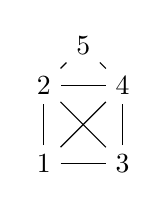
\begin{tikzpicture}[scale=0.5]
    \node (1) at (-1,-1) {$1$};
    \node (2) at (-1,1) {$2$};
    \node (3) at (1,-1) {$3$};
    \node (4) at (1,1) {$4$};
    \node (5) at (0,2) {$5$};
    \draw[-] (1) -- (2);
    \draw[-] (2) -- (3);
    \draw[-] (3) -- (4);
    \draw[-] (4) -- (2);
    \draw[-] (2) -- (5);
    \draw[-] (5) -- (4);
    \draw[-] (4) -- (1);
    \draw[-] (1) -- (3);
\end{tikzpicture}}}\right),\qquad H\colon\left(\vcenter{\hbox{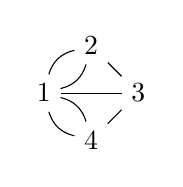
\begin{tikzpicture}[scale=0.6]
\node (1) at (-1, 0) {$1$};
\node (2) at (0, 1) {$2$};
\node (3) at (1,0) {$3$};
\node (4) at (0,-1) {$4$};
\draw[-] (1) -- (3);
\path [-] (1) edge[bend right=-30](2); 
\path [-] (1) edge[bend right=30](2); 
\path [-] (1) edge[bend right=-30](4); 
\path [-] (1) edge[bend right=30](4);
\draw[-] (3) -- (2);
\draw[-] (4) -- (3);
\end{tikzpicture}}}\right)
\end{equation}
\end{ex}
\begin{defi}[Face Graph]
    Let $M = (\mathcal{V}_M, \mathcal{F}_M)$ be a mesh and
    \begin{align*}
        \mathcal{E} = \left\{(f_1,f_2)\in\mathcal{F}_G^2: \vert f_1\cap f_2\vert =2\right\}
    \end{align*}
    The face graph of $M$ is the graph $(\mathcal{F}_M,\mathcal{E})$.
\end{defi}
\begin{ex} The face graph of the tetrahedron is given by
    \begin{equation}\label{eq:sample_g}
    G\colon\left(\vcenter{\hbox{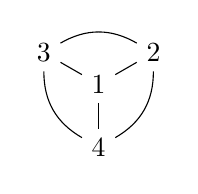
\begin{tikzpicture}[scale=0.8]
    \node (1) at (0,0) {$1$};
    \node (2) at (0.87,0.5) {$2$};
    \node (3) at (-0.87,0.5) {$3$};
    \node (4) at (0,-1) {$4$};
    \draw[-] (1) -- (2);
    \draw[-] (1) -- (3);
    \draw[-] (1) -- (4);
    \path[-] (2) edge[bend right=30] (3);
    \path[-] (3) edge[bend right=30] (4);
    \path[-] (4) edge[bend right=30] (2);
\end{tikzpicture}}}\right)
\end{equation}
\end{ex}
The face graph of a given mesh can be constructed by algorithm \ref{alg:facegraph}.
\begin{algorithm}\label{alg:facegraph}
    \SetKwInOut{Input}{Input}
    \SetKwInOut{Output}{Output}

    \Input{A mesh $M = (\mathcal{V}_M, \mathcal{F}_M=\{f_1,f_2,f_3\ldots\})$}
    \Output{The adjacency matrix of the face graph of the mesh $M$}
    \caption{Construction of the face graph of a given mesh}
    $G := 0\in\R^{F_M\times F_M}$\;
    \For{$i=1$ \KwTo $F_M$}
    {
        $neighbors := 0$\;
        \For{$j=1$ \KwTo $F_M$}
        {
            \If{$neighbors = 3$}{
            \textbf{break}\;
            }
            \If{$\vert f_i\cap f_j\vert = 2$ \normalfont{\textbf{and}} $i\neq j$}{
            $G_{ij} \leftarrow 1$\;
            $neighbors \leftarrow neighbors + 1$\;
            }
        }
    }
    \Return{$G$}
\end{algorithm}
Since this algorithm loops over the faces of the mesh in a nested way, the complexity of it lies in $O(F_M^2)$. As this runtime complexity has the consequence of the algorithm being very slow at execution for somewhat large meshes, the face graph is computed dynamically by \texttt{maniflow.mesh.Mesh.faceGraph}.
\newpage
\subsection{A first application: \texttt{maniflow.mesh.utils.connectedComponents}}
The method \texttt{maniflow.mesh.utils.connectedComponents} decomposes the given mesh into its connected components. Now that we have an algorithm with which to compute the face graph, the connected components of a mesh can now be identified as the connected components of the face graph. These can be determined via the breadth-first traversal of the face graph. 
\begin{algorithm}\label{alg:components}
    \SetKwInOut{Input}{Input}
    \SetKwInOut{Output}{Output}

    \Input{A mesh $M = (\mathcal{V}_M, \mathcal{F}_M=\{f_1,f_2,f_3\ldots\})$}
    \Output{The connected components of the mesh $M$}
    \caption{Construction of the face graph of a given mesh}
    Compute the adjacency matrix $G$ using \ref{alg:facegraph}\;
    $start := 1$\;
    $n := 1$\;
    \While{$\mathcal{F}_M\neq\emptyset$}{
        Compute a breadth first traversal sequence $T_n \leftarrow \{f_{start}, f_b,f_c,\ldots\}\subseteq\mathcal{F}_M$\;
        $n \leftarrow n+1$\;
        $\mathcal{F}_M\leftarrow \mathcal{F}_M\setminus T_n$\;
        Set $1< start\leq F_M$ such that $f_{start}\in\mathcal{F}_M$\;
    }
    
    \Return{$T_1$, $T_2$, $\ldots$}
\end{algorithm}
\paragraph{Runtime analysis.} The algorithm \ref{alg:facegraph} has a runtime complexity which lies in $O(F_M^2)$. The breadth-first traversal on the face graph has a runtime\footnote{Since on a graph with the number of vertices being $V$ and the number of edges being $E$ the breadth first search has a complexity of $O(E + V)$. As every face has at most three neighbors we obtain the given runtime complexity.} complexity of $O(F_G + 3\cdot F_G) = O(F_G)$. The computation of $\mathcal{F}_M\setminus T_n$ has also quadratic complexity $O(\vert\mathcal{F}_M\vert^2)$. Thus the overall complexity of algorithm \ref{alg:components} lies in $O(F_G^2)$.
\begin{ex}
    In this example we analyse the connected components of the teapot from \texttt{examples/teapot.obj}. The teapot is displayed in figure \ref{fig:teapot}.
    \begin{figure}[h]
        \centering
        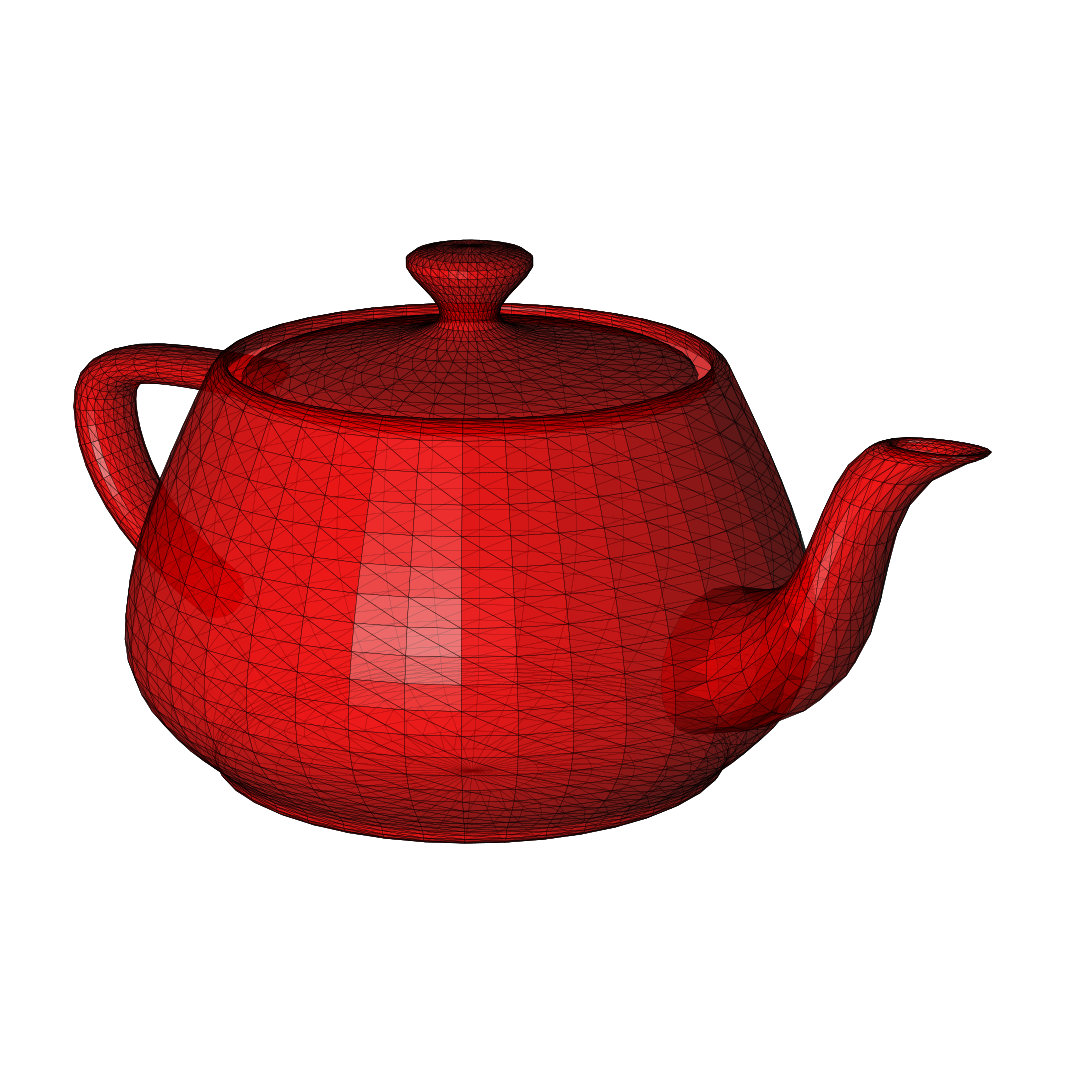
\includegraphics[scale=0.15]{img/teapot.png}
        \caption{The teapot from \texttt{examples/teapot.obj}}
        \label{fig:teapot}
    \end{figure}
    \newline\noindent The connected components can be computed using the following code
    \begin{lstlisting}
from maniflow.mesh import Mesh
from maniflow.mesh.obj import OBJFile
from maniflow.mesh.utils import connectedComponents, coincidingVertices

teapot = OBJFile.read("examples/teapot.obj")
coincidingVertices(teapot)
components = connectedComponents(teapot)

for i, component_list in enumerate(components):
    component = Mesh.fromFaceList(teapot, *component_list)
    OBJFile.write(component, "teapot" + str(i + 1) + ".obj")
    \end{lstlisting}
    \begin{figure}[ht]
    \centering
    \subfloat[The lid of the teapot]{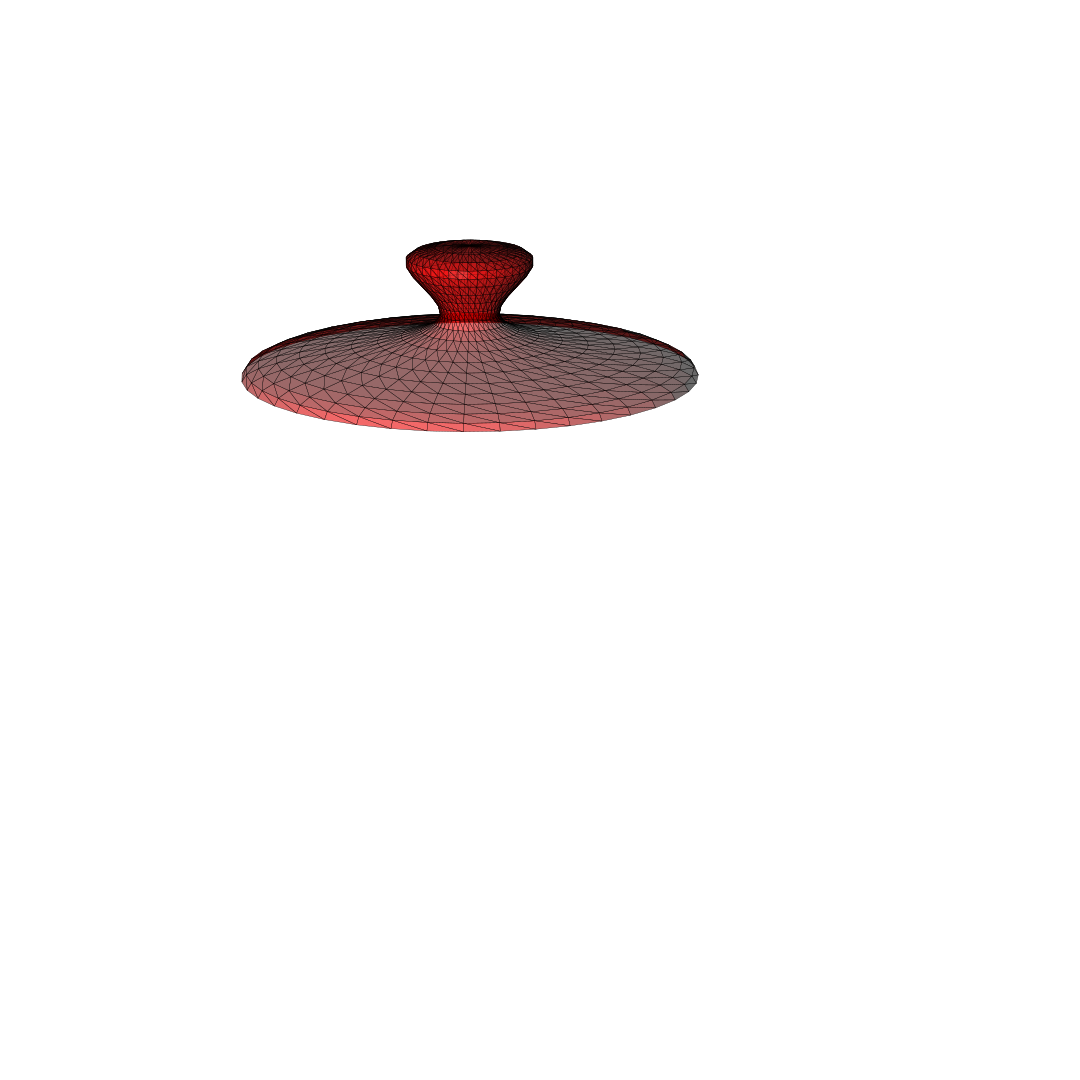
\includegraphics[width=0.4\textwidth]{img/teapot1.png}}\hfil
    \subfloat[The handle of the teapot]{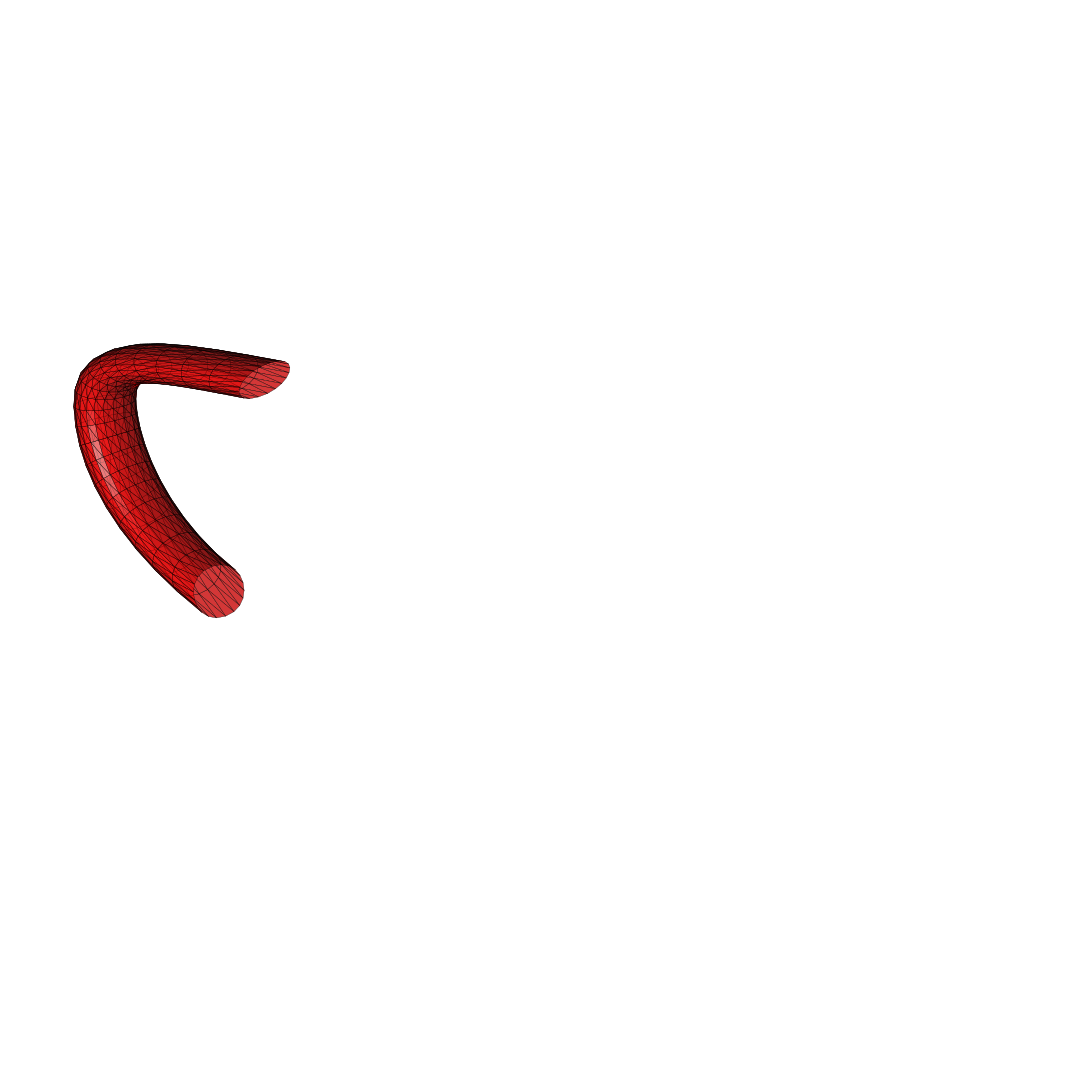
\includegraphics[width=0.4\textwidth]{img/teapot2.png}}\hfil\\
    \subfloat[The body of the teapot]{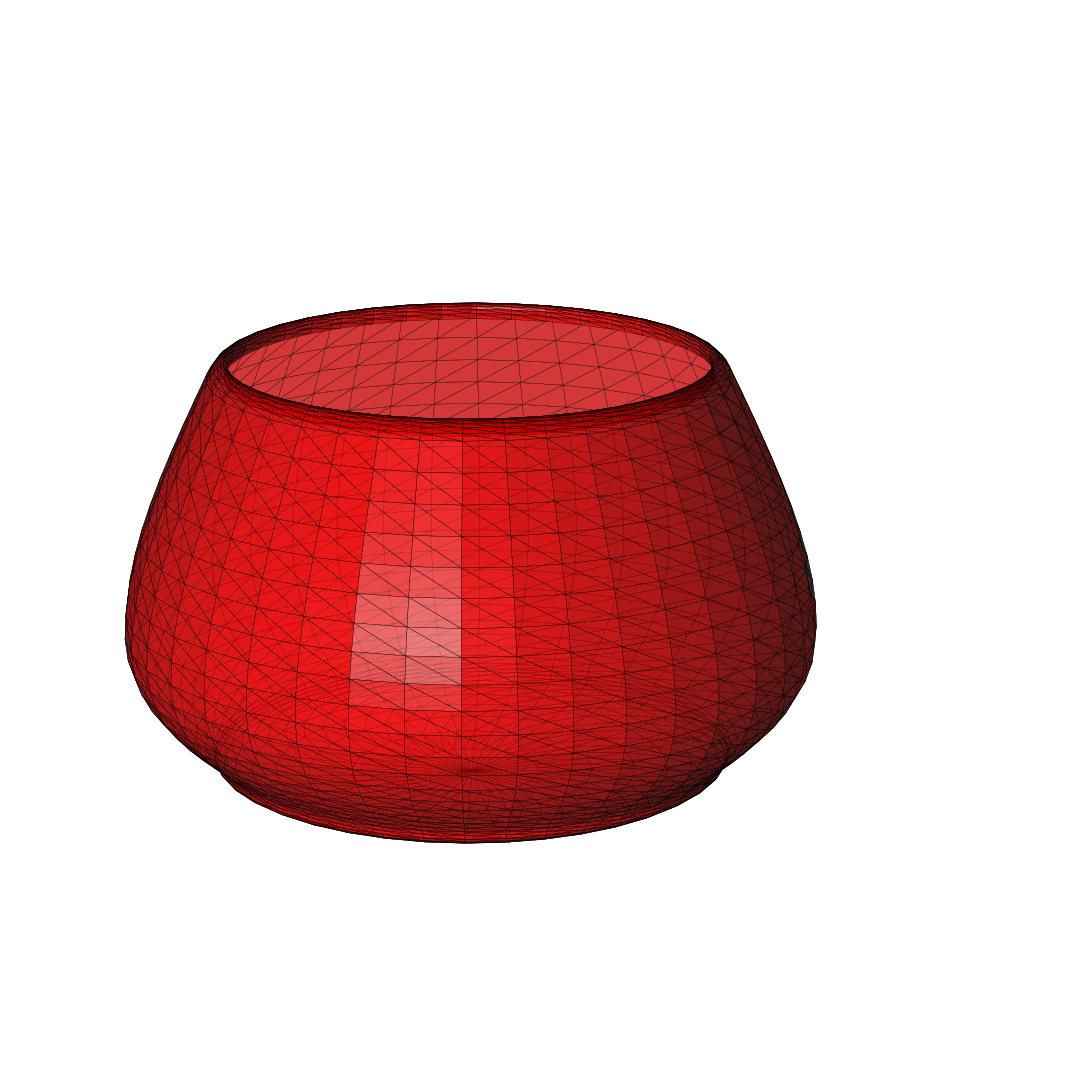
\includegraphics[width=0.4\textwidth]{img/teapot3.png}}\hfil
    \subfloat[The spout of the teapot]{
\includegraphics[width=0.4\textwidth]{img/teapot4.png}}\hfil
    \caption{The connected components of the teapot}
    \label{fig:einsteinex}
\end{figure}
\end{ex}
\end{document}

\section{Rendering meshes}
\maniflow{} employs rasterization, a fundamental technique in computer graphics, to render meshes. This process involves projecting each face of the mesh onto the viewing plane. The \texttt{maniflow.render.camera.Camera} class encapsulates the necessary matrices and operations for this projection.

\maniflow{} provides three renderers whose functionality is basically the same. Firstly, the vertices of each surface of the mesh are projected onto the display plane by means of said projections. These projected polygons (triangles) are then drawn. The only difference between the three renderers provided is how the triangles are drawn.

\subsection{The camera system}
Standard OpelGL matrices... \cite{Teschner}

\section{Geometry}
\subsection{Curvature}
\begin{ex}[Gauss-Bonnet Theorem] For a compact $2$-manifold with $\partial M = \emptyset$ we have
    \begin{align*}
        \int_M K\mathrm{d}A = 2\pi\chi(M).
    \end{align*}
    Analogously we can state a discretized version:
    \begin{align*}
        \sum_{i\in \mathrm{vert}(M)}K_i = 2\pi\chi(M).
    \end{align*}
\end{ex}
\section{Coinciding Vertices}
The \texttt{coincidingVertices} function is an essential component in mesh processing algorithms, designed to identify and handle vertices with the same coordinates. This functionality becomes crucial in scenarios where mesh data contains overlapping vertices due to precision limitations or data noise.\\

An example for the usage of \texttt{coincidingVertices} can be found in \autoref{subsec:connected_Components}. While we can see the four components of the teapot neatly displayed in \autoref{fig:teapotcomps} this is after identifying similar vertices with each other. Just taking the original data and looking at the connected components results in a surprising amount of components.

\begin{lstlisting}[language=Python, caption={Connected components with and without \texttt{coincidingVertices}}, label={lst:coincidingVertices}]
from maniflow.mesh import Mesh
from maniflow.mesh.obj import OBJFile
from maniflow.mesh.utils import connectedComponents, coincidingVertices

teapot = OBJFile.read("examples/teapot.obj")  # reading the mesh from memory

print(f"Without coinciding the vertices there are {len(connectedComponents(teapot))} components.")

coincidingVertices(teapot)  # identifying and collapsing coinciding vertices
print(f"After coinciding the vertices there are {len(connectedComponents(teapot))} components.")
\end{lstlisting}

\begin{lstlisting}[escapeinside={<@}{@>}]
Without coinciding the vertices there are 19 components.
After coinciding the vertices there are 4 components.
\end{lstlisting}

What happened here is that the four intuitively expected components had been designed as quarters and then assembled. To the eye it does not make a difference but for the code it does.

Looking at some of the $19$ components we see that the teapot seems to have been created by having parts of a repeating object, say the floor of the teapot where there are four quarters of, being moved and turned to fit together. For example, by running \autoref{lst:teapot_four_components} without \texttt{coincidingVertices} in line 6 we end up getting said $19$ components as .obj-files. Then running

\begin{lstlisting}[language=Python, caption={Visualizing the parts of the bottom of the teapot}, label={lst:teapot_btm_parts}]
from maniflow.mesh.parameterized import *
from maniflow.mesh.obj import OBJFile
from maniflow.render import SVGPainterRenderer
from maniflow.render.scene import *

# 4 times as we have four parts of the bottom of the teapot
for i in range(4):
    teapot_btm = OBJFile.read(f"teapot{16+i}.obj")
    # Invert orientation for colour visibility
    for j in range(teapot_btm.f):
        teapot_btm.faces[j].vertices = teapot_btm.faces[j].vertices[::-1]
    # Setting up renderer
    teapot_btm.setStyle('red')
    camera = Camera(position(10,-20,5), target=(0, -0.7, 0))
    scene = Scene(camer=camera, width=400, height=400, light=np.array([10, -1.5, 50]
    renderer = SVGPainterRenderer(scene)
    # Take image and save it
    image = renderer.render(teapot_btm)
    image.save_svg(f"teapot_part{i+1}_render.svg")
\end{lstlisting}

gets us the four components that form the bottom of the teapot in \autoref{fig:teapot_parts}:

\begin{figure}[H]%
\scalebox{.75}{
\centering
\subfloat[First part]{\includesvg[width=0.35\textwidth]{img/teapot_part2_render.svg}}\qquad
\subfloat[Second part]{\includesvg[width=0.25\textwidth]{img/teapot_part1_render.svg}}\qquad
\subfloat[Third part]{\includesvg[width=0.25\textwidth]{img/teapot_part3_render.svg}}\qquad
\subfloat[Forth part]{\includesvg[width=0.35\textwidth]{img/teapot_part4_render.svg}}\qquad}
\caption{The quarters of the bottom of the teapot.}
\label{fig:teapot_parts}
\end{figure}

Similarly, when we take a look at the moebius strip generated from a grid, we note that while the ends have the same points they still are not glued together. Again, to the eye there is no difference but topologically the moebius strip created from the grid is then just a plain with Euler Characteristic $1$. Yet, it is well-known that an actual moebius strip has an Euler Characteristic of $0$. Using \texttt{coincidingVertices} we can glue those loose ends together to get:

\begin{lstlisting}[language=Python, caption={Euler Characteristic of the moebius strip with and without \texttt{coincidingVertices}}, label={lst:coincidingVertice_eulers}]
import numpy as np
from maniflow.mesh.parameterized import *

@VertexFunction
def moebius(vertex):
    x = vertex[0]
    y = vertex[1]
    x0 = np.cos(x) * (1 + (y / 2) * np.cos(x / 2))
    x1 = np.sin(x) * (1 + (y / 2) * np.cos(x / 2))
    x2 = (y / 2) * np.sin(x / 2)
    return np.array([x0, x1, x2])

u = Grid((0, 2 * np.pi), (-1, 1), 30, 10)  # create a high resolution grid
moebiusMesh = moebius(u)

print(f"Euler Characteristic before coincidingVertices: {eulerCharacteristic(moebiusMesh)}")
coincidingVertices(moebiusMesh)
print(f"Euler Characteristic after coincidingVertices: {eulerCharacteristic(moebiusMesh)}")
\end{lstlisting}

\begin{lstlisting}[escapeinside={<@}{@>}]
Euler Characteristic before coincidingVertices: 1
Euler Characteristic after coincidingVertices: 0
\end{lstlisting}

\subsection{The Upper Triangular Approach}
The old version of \texttt{coincidingVertices} utilizes an approach with a time complexity of $O(n^2)$, where $n$ represents the number of vertices in the mesh. This stems from iterating twice through all or at least a linearly decreased subset of the vertex data. While being naive in its concept there are a few tweaks that improve the algorithm, more than halving its runtime. That of course is not as good as it sounds given that we have a quadratic runtime nature.

It starts by initializing empty data structures, iterates through each vertex to detect coinciding vertices, merges them into a single vertex, and updates the mesh accordingly. To reduce computational power needed this naive approach is improved by the simple fact that if $a == b$ then also $b == a$, so this halves the amount of iteration steps in a double for-loop leading to these computations. This leaves us with an upper triangular form where we only have to check the following indices but not the previous as those where checked before. E.g. when checking whether the third vertex can be identified with another vertex we can start at the fourth vertex since, say, the check against the second vertex already happened when we previously check for identities with the second vertex. The resulting checks can be visualized in a matrix looking similar to this
\begin{center}
\begin{tabular}{|*{7}{c|}}
                               \hline
    & 1 & 2 & 3 & 4 & 5 & n \\ \hline
  1 &   & X & X & \checkmark & X & X \\ \hline
  2 &   &   & X & - & X & X \\ \hline
  3 &   &   &   & - & X & X \\ \hline
  4 &   &   &   &   & - & - \\ \hline
  5 &   &   &   &   &   & X \\ \hline
  n &   &   &   &   &   &   \\ \hline
\end{tabular}
\end{center}

where the 'X' implies a comparison to be done and the '\checkmark' denotes, in this case, that the first vertex and the fourth vertex are the same point with regard to our tolerance. This results in canceling all checks for (row) and against (column) the fourth vertex as this check has been done for the identical first vertex already, indicated by '-'. Because of this canceling we get a best case scenario of $O(n)$ that is if all vertex are identified to be the same point. After one iteration through all of them we have identified them all with the first vertex resulting in not going through their rows and columns. This leaves only the first $n$ checks.
\begin{center}
\begin{tabular}{|*{7}{c|}}
                               \hline
    & 1 & 2 & 3 & 4 & 5 & n \\ \hline
  1 &   & \checkmark & \checkmark & \checkmark & \checkmark & \checkmark \\ \hline
  2 &   &   & - & - & - & - \\ \hline
  3 &   &   &   & - & - & - \\ \hline
  4 &   &   &   &   & - & - \\ \hline
  5 &   &   &   &   &   & - \\ \hline
  n &   &   &   &   &   &   \\ \hline
\end{tabular}
\end{center}

\subsubsection{Bubblesort by accident}
Without realizing at the time of first implementation the upper triangular approach is equivalent to the Bubblesort sorting algorithm. As a reminder, Bubblesort also first iterates through all elements. At the end of the iteration one of the elements is at its proper place. Afterwards, it repeats with the next iteration but this time it can leave out checking said element. Bubblesort functions in the following way:\\
\begin{algorithm}[H]
    \SetAlgoLined
    \SetKwInOut{Input}{Input}
    \SetKwInOut{Output}{Output}

    \Input{List of sortable elements}
    \Output{Sorted List}
    \caption{Bubblesort}
    \label{alg:bubblesort}
    \KwData{List}
    \For{i := 1 to n - 1}{
        Set swapped flag to False\;
        \For{j :=1 to n - i}{
            \If{j-th element is smaller than (j-1)-th element}{
                Swap the two elements\;
                Set swapped flag to True\;
            }
        }
        \If{swapped flag is set to False}{
            Stop\;
        }
    }
\end{algorithm}

This is essentially the algorithm used for the upper triangular approach with the only difference being the direction of the inner loop, i.e. for the $i$-th row it starts from the at $i+1$ and ends at the end $n$ for the upper triangular but Bubblesort always starts at the beginning and ends at $n-i$.\\
The advantage we get now is that the runtime performance of Bubblesort is well known. Having the same structure this means that our upper triangular approach we ca not only confirm the performance mentioned above, that is $O(n)$ in the best case and $O(n^2)$ in the worst case, but also get the average case from Bubblesort, which is $O(n^2)$ as well.

\subsection{Time to sort - Using Timsort to speed things up}
The updated version of \texttt{coincidingVertices} employs a more efficient approach compared to the old version. It starts by creating an empty list \texttt{extVertList} and copies the mesh's faces into \texttt{faceList}. It then iterates through each face and its vertices, adding the $j$-th vertex in the $i$-th face along with the information on $i$ and $j$ to \texttt{extVertList}. Next, it sorts \texttt{extVertList} by the first element (the vertex coordinates) using Python's Timsort algorithm, resulting in a stable sorting with an average time complexity of $O(n\log n)$. Overall, timsort is linear with $O(n)$ in the best case as it is an adaptive sorting algorithm, and capped in the worst case at $O(n\log n)$.

The function then initializes an empty list \texttt{vertList} and iterates through all entries of \texttt{extVertList}. For each entry \texttt{v}, it checks if \texttt{vertList} is empty or if the vertex is not close to the previous one. If so, it adds the vertex to \texttt{vertList}. Additionally, it updates the vertices in \texttt{faceList} based on the indices in \texttt{vertList}, ensuring that vertices with the same coordinates are identified and glued together.

\begin{algorithm}[H]
    \SetAlgoLined
    \SetKwInOut{Input}{Input}
    \SetKwInOut{Output}{Output}

    \Input{Mesh}
    \Output{Mesh with identified vertices}
    \caption{coincidingVertices Timsort}
    \label{alg:coincidingVertices_timsort}
    \KwData{mesh}
    Initialize list 'extVertList'\;
    Create work copy 'faceList' of the faces of the mesh\;
    \For{every face in 'faceList'}{
        \For{every vertex in the face}{
            Add [coordinate of vertex, index of face, index of vertex] to 'extVertList'\;
        }
    }
    Sort 'extVertList' by coordinates, starting with the first\;
    Initialize list 'vertList'\;
    \For{every entry 'v' in 'extVertList'}{
        \If{either 'vertList' is empty or the latest entry of 'vertList' is not close to 'v'}{
            Add 'v' to 'vertList'\;
        }
        Update the vertex in the face referenced in 'v'\;
    }
    Copy the values of 'faceList' into the initial mesh\;
\end{algorithm}

Note that the definition of closeness is not the standard metric but whether the vertices can be fitted into a box of size $2\textit{atol} \times 2\textit{atol} \times 2\textit{atol}$. While not as intuitive as a simple distance between the points in the three dimensional, this allows us to use the a sorting algorithm since the vertices have to be within \texttt{atol} on \textit{all} three coordinate axis. This means we can start looking at the first coordinate, compare that and, if it is within tolerance, we can continue with the second and third if needed. Hence, we can sort the first coordinates (if equal then go by the second, etc.). This approach can be used, as we did, to implement a fast algorithm that only needs to check the previous vertex for equality since it is the closest yet tested vertex, at least on the first coordinate. And since we are checking not the Euclidean distance between points but have this box approach all of the coordinates have to be contained. Thus, we can stop if the first coordinate is not close. If it is, we check for the second coordinate. As these are sorted as well, the latest entry to \texttt{vertList} has to be the closest to the currently checked vector in the second coordinate as well, given closeness in the first. This can be applied to the third coordinate as well.

By using not only the fast sorting of timsort but also being able to just check against a single different point (so comparing up to three different floats) this algorithm is very fast and efficient. Since we just iterate once through the faces and their three respective vertices ($3n$ operations), sorting with on average (and even in the worst case) $O(n\log n)$ and then iterate again only once though the list \texttt{extVertList} of length $n$, we end up with $O(3n)+O(n\log n)+O(n)=O(n\log n)$ as overall runtime.

\subsection{Time comparison}
A direct comparison can be drawn by using the \texttt{timeit}-package in Python. Since \texttt{coincidingVertices} normally overwrites the mesh given in the parameter we need to make adjustments to the functions for example introducing a variable called 'dummy' that is written into instead of the original mesh. It is only used for this writing of data and the timing method applied here.

The comparison will be drawn between the two implementations using the teapot OBJ-file already present. It consists of $3644$ vertices which both functions will bring down to $3241$. This is a decrease of about about 11.1\% or one in every nine vertices being identified with another vertex.

As the main load of the computation is on the naive double-looping (upper triangle) and the sorting algorithm we can expect the other calls in the functions such as list manipulations and calls to stored data to be insignificant with the difference in performance being $O(n^2)$ and $O(n\log n)$ on average for a relatively (to simpler shapes) large $n=3644$.

\begin{lstlisting}[language=Python, caption={Timing Comparison between Upper Triangular and Timesort Approach}, label={lst:timing_comparison}]
from timeit import default_timer as timer

teapot = OBJFile.read("examples/teapot.obj")

repetitions = 10    # coincidingVertices_old is SIGNIFICANTLY slower than the newer version, choose repetitions accordingly
time_a = 0
time_b = 0

# cumulated time for the upper triangular method
for i in range(repetitions):
    start = timer()
    coincidingVertices_old(teapot)
    end = timer()
    time_a = time_a + (end - start)

# cumulated time for the timsort method
for i in range(repetitions):
    start = timer()
    coincidingVertices_new(teapot)
    end = timer()
    time_b = time_b + (end - start)

print(f"Upper Triangle Approach execution time avg.: {time_a/repetitions} seconds")
print(f"Sorting Algorithm Approach execution time avg.: {time_b/repetitions} seconds")
\end{lstlisting}

The code outputs the following result
\begin{lstlisting}[escapeinside={<@}{@>}]
Upper Triangle Approach execution time avg.: 81.20345090379979 seconds
Sorting Algorithm Approach execution time avg.: 0.33098463589976745 seconds
\end{lstlisting}

This result is completely within expectation and still depicts nicely how even for a not extremely large $n=3644$ we already need about $245$ times longer with the upper triangular than with timesort. Since we are working with a non-small $n$ the quadratic nature of the upper triangular approach weights heavy on the runtime to the point that using for the renderer the upper triangular approach is simply not feasible.

\subsection{Further thoughts}
With this speedy approach come limitations, though. The algorithm does not care for relative closeness, all it looks at is \textit{whether} it is within \texttt{atol} but not \textit{how} close the vertices are when within this tolerance. This can lead to cases where for three points $[a, b, c]$ with $a$ and $b$ being close (as in within the \texttt{atol}-box) and $b$ and $c$ being close, but not $a$ and $c$.

The algorithm starts from $a$ and checks against $b$. They are close so it identifies $a$ and $b$ with coordinates of $a$. But then $a$ and $c$ are not close so they are not the same (w.r.t. the program) even though $b$ and $c$ might have been closer to each other than $a$ and $b$, see \autoref{fig:coinciding_vertices_a_start}. We hence can have non-optimal identifications for vertices which, again, is a trade-off that is made for increased computational efficiency.\\

\begin{figure}[t]
    \centering
    \subfloat[Identifying $b$ with $a$ as we start with $a$]{
        \centering
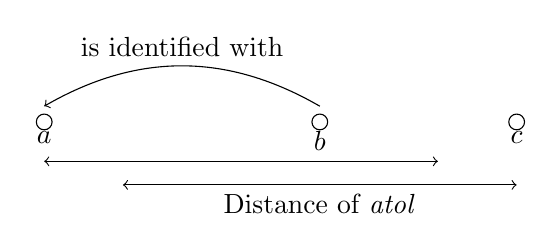
\begin{tikzpicture}
    % Define points a, b, and c
    \coordinate (a) at (0,0);
    \coordinate (b) at (3.5,0);
    \coordinate (c) at (6,0);

    % Draw circles around points a, b, and c
    \draw (a) circle [radius=0.1] node[below] {$a$};
    \draw (b) circle [radius=0.1] node[below] {$b$};
    \draw (c) circle [radius=0.1] node[below] {$c$};

    % Draw distance indicator
    \draw[<->] ([yshift=-0.5cm]a) -- node[below] {} ([xshift=-1cm,yshift=-0.5cm]c);
    \draw[<->] ([xshift=1cm,yshift=-0.8cm]a) -- node[below] {Distance of \textit{atol}} ([yshift=-0.8cm]c);

    % Draw curved arrow from b to a
    \draw[->, bend right] ([yshift=0.2cm]b) to node[above] {is identified with} ([yshift=0.2cm]a);
\end{tikzpicture}
}
\hfill
    \subfloat[$a$ and $c$ are not close enough for identification]{
    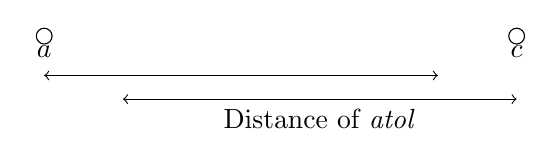
\begin{tikzpicture}
    % Define points a, b, and c
    \coordinate (a) at (0,0);
    \coordinate (c) at (6,0);

    % Draw circles around points a, b, and c
    \draw (a) circle [radius=0.1] node[below] {$a$};
    \draw (c) circle [radius=0.1] node[below] {$c$};

    % Draw distance indicator
    \draw[<->] ([yshift=-0.5cm]a) -- node[below] {} ([xshift=-1cm,yshift=-0.5cm]c);
    \draw[<->] ([xshift=1cm,yshift=-0.8cm]a) -- node[below] {Distance of \textit{atol}} ([yshift=-0.8cm]c);
\end{tikzpicture}
}
    \caption{Coinciding the vertices $a,b,c$ when starting with $a$}
    \label{fig:coinciding_vertices_a_start}
\end{figure}
%
\begin{figure}[t]
    \centering
    \subfloat[Identifying $a$ with $b$]{
        \centering
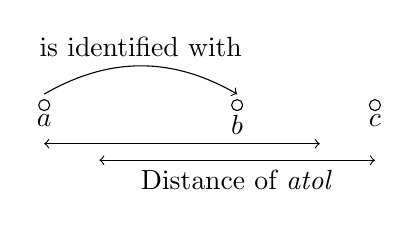
\begin{tikzpicture}[scale=0.7]
    % Define points a, b, and c
    \coordinate (a) at (0,0);
    \coordinate (b) at (3.5,0);
    \coordinate (c) at (6,0);

    % Draw circles around points a, b, and c
    \draw (a) circle [radius=0.1] node[below] {$a$};
    \draw (b) circle [radius=0.1] node[below] {$b$};
    \draw (c) circle [radius=0.1] node[below] {$c$};

    % Draw distance indicator
    \draw[<->] ([yshift=-0.7cm]a) -- node[below] {} ([xshift=-1cm,yshift=-0.7cm]c);
    \draw[<->] ([xshift=1cm,yshift=-1cm]a) -- node[below] {Distance of \textit{atol}} ([yshift=-1cm]c);

    % Draw curved arrow from b to a
    \draw[<-, bend right] ([yshift=0.2cm]b) to node[above] {is identified with} ([yshift=0.2cm]a);
\end{tikzpicture}
}
\hfill
    \subfloat[Identifying $c$ with $b$]{
    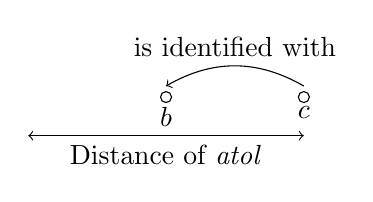
\begin{tikzpicture}[scale=0.7]
    % Define points a, b, and c
    \coordinate (a) at (0,0);
    \coordinate (b) at (3.5,0);
    \coordinate (c) at (6,0);

    % Draw circles around points a, b, and c
    \draw (b) circle [radius=0.1] node[below] {$b$};
    \draw (c) circle [radius=0.1] node[below] {$c$};

    % Draw distance indicator
    \draw[<->] ([xshift=1cm,yshift=-0.7cm]a) -- node[below] {Distance of \textit{atol}} ([yshift=-0.7cm]c);
    \draw[->, bend right] ([yshift=0.2cm]c) to node[above] {is identified with} ([yshift=0.2cm]b);
\end{tikzpicture}
}
\hfill
\subfloat[Only $b$ left, nothing to do]{
        \centering
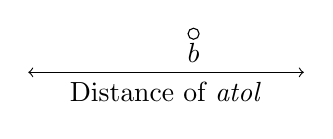
\begin{tikzpicture}[scale=0.7]
    % Define points a, b, and c
    \coordinate (a) at (0,0);
    \coordinate (b) at (3.5,0);
    \coordinate (c) at (6,0);

    % Draw circles around points a, b, and c
    \draw (b) circle [radius=0.1] node[below] {$b$};

    % Draw distance indicator
    \draw[<->] ([xshift=0.5cm,yshift=-0.7cm]a) -- node[below] {Distance of \textit{atol}} ([xshift=-0.5cm,yshift=-0.7cm]c);
\end{tikzpicture}
}
    \caption{Coinciding vertices this time starting with $b$}
    \label{fig:coinciding_vertices_b_start}
\end{figure}

Also note that the implemented function is iterating through the points in order that they are listed. Depending on the order in the list we can have different results visualized by comparing \autoref{fig:coinciding_vertices_a_start} and \autoref{fig:coinciding_vertices_b_start}. So if we were to start from vertex $b$ because it is mentioned before $a$ and $c$, this means that we check whether $b == a$ and not $a == b$, then $b$ and $a$ would be identified in the point $b$ and not $a$. As $b$ and $c$ are close as well, this would again be coincided in $b$ resulting in one ($b$) and not two ($a$ and $c$) remaining vertices originating from the initial three.

This could lead to the case that, as the upper triangle approach is simply iterating through the vertices in the mesh beginning from the first while the sort approach may change the order for the sorting, we may in some rarer cases end up with a different amount of vertices for the different implementations. The deviating numbers of vertices could become an issue if we were to use both approach alongside each other, which we are not. The upper triangle matrix was an early, naive approach to solve the problem for a small number of vertices where the $O(n^2)$ did not affect the computational time significantly. It will be completely replaced by the sort approach as the used timsort is better on average and in the worst-case with $O(n\log n)$ and equal in the best-cast (linear).\\

As another note, timsort is a stable sorting algorithm that means the even if we had points that are exactly the same the order in which they are mentioned would be kept so there are no differences if applied at different times despite of the shortcomings mentioned above.
\section{Mesh simplification}
Mesh simplification is a fundamental technique in computer graphics and computational geometry, employed to optimize the performance of various applications, such as 3D modeling, simulation, and rendering. By reducing the complexity of a mesh while preserving its essential features, mesh simplification achieves a balance between computational efficiency and visually staying true to the original.

The process of mesh simplification involves iteratively removing vertices, edges, or faces from the original mesh while minimizing the perceptible loss of detail. Various algorithms and methodologies have been developed to accomplish this task, ranging from straightforward decimation techniques to sophisticated error-driven approaches.

Furthermore, mesh simplification is not only beneficial for real-time rendering and interactive applications but also plays a crucial role in data storage, transmission, and manipulation. By generating simplified representations of complex meshes, the storage requirements are minimized, facilitating efficient data exchange and manipulation across different platforms and devices.

\subsection{Implemented Approach}
\subsubsection{Approach to Mesh Simplification}
In our approach we deploy vertex contraction as described in \cite{GarlandHeckbert}. This way we cut down on the amount of vertices and hence faces. Technically, also the amount of edges is reduced but in our project the edges are only considered via vertices and faces.\\
The procedure has several steps depicted below as pseudocode:

\begin{algorithm}[H]
    \SetAlgoLined
    \SetKwInOut{Input}{Input}
    \SetKwInOut{Output}{Output}

    \Input{mesh: A mesh}
    \Output{The simplified mesh}
    \caption{Mesh Simplification}
    \label{alg:mesh_simplification}
    \KwData{mesh}
    
    Clean the mesh to ensure consistency\;
    Initialize an empty list for Q values\;
    \For{each vertex in the mesh}{
        Compute the initial Q value for the vertex\;
        Add the computed Q value to the list\;
    }

    Initialize an empty validity matrix for vertex pairs\;
    \For{each face in the mesh}{
        Mark vertex pairs sharing an edge as valid in the validity matrix\;
    }

    Initialize an empty cost dictionary\;
    \For{each pair of valid vertices}{
        \If{the normals of the adjacent faces don't flip after contraction}{
            Calculate the cost of contraction and add it to the dictionary\;
        }
    }

    Sort the cost dictionary based on cost values\;

    Initialize a reduction goal based on desired reduction percentage\;
    \While{the number of faces in the mesh is greater than the reduction goal}{
        Choose the vertex pair with the lowest cost from the dictionary\;
        Update the mesh by contracting the chosen vertex pair\;
        Update the validity matrix and cost dictionary accordingly\;
    }

    Remove redundant vertices and faces from the mesh\;
    \Return{the simplified mesh}\;
\end{algorithm}

After getting rid of redundant vertices by applying \texttt{coincidingVertices} we want to compute a characteristic matrix \(\bm{Q}\) for each vertex. This characteristic will help us in computing the optimal contraction point. Say, we have a vector \(\bm{v}=[v_x, v_y, v_z, 1]^T\). Then the error at \(\bm{v}\) is denoted by
\begin{align*}
    \Delta(\bm{v})&=\sum_{\bm{p}\text{ is a plane of }\bm{v}}(\bm{v}^T\bm{p})(\bm{p}^T\bm{v})\\
    &=\bm{v}^T\left(\sum_{\bm{p}\text{ is a plane of }\bm{v}}\bm{K}_{\bm{p}}\right)\bm{v}
\end{align*}
with \(\bm{K}_{\bm{p}}=\bm{p}\bm{p}^T\) being called the fundamental quadric error. Since \(\bm{p}\) is a plane given by the equation
\begin{equation*}
    ax+by+cz+d=0,\hspace{4pt}a^2+b^2+c^2+d^2=1
\end{equation*}
we get that \(\bm{K}_{\bm{p}}\) is a \(4\times4\)-matrix.\\
The characteristic matrix \(\bm{Q}\) mentioned before is then the sum over fundamental quadric errors. We get that
\begin{equation}\label{eq:contraction_cost}
    \Delta(\bm{v})=\bm{v}^T\bm{Q}\bm{v}
\end{equation}
and choose that for two vertices $\bm{v_1}$ and $\bm{v_2}$ and their respective $\bm{Q_1}$ and $\bm{Q_2}$ we have $\bar{\bm{Q}}=\bm{Q_1}+\bm{Q_2}$ in their contraction point $\bar{\bm{v}}$. Minimizing the error $\Delta(\bar{\bm{v}})$, we use that it is quadratic. That implies that the minimal solution to this problem is linear, meaning that we set the partial derivatives of the error to zero. The problem can be reformulated to
\begin{equation*}
    \bar{\bm{v}}=\begin{pmatrix}
        q_{11} &q_{12} &q_{13} &q_{14}\\
        q_{21} &q_{22} &q_{23} &q_{24}\\
        q_{31} &q_{32} &q_{33} &q_{34}\\
        0   &0  &0  &1
    \end{pmatrix}^{-1}\begin{pmatrix}
        0\\0\\0\\1
    \end{pmatrix}
\end{equation*}
where $q_ij$ is the element of the $i$-th row and $j$-th column of $\bar{\bm{Q}}$.

If the matrix is not invertible then we want to choose one of the two initial vertices or their midpoint as new point of contraction. This depends on whichever of the three is minimizing the error best among them.\\

For the next step we want to get \textit{valid pairs} of vertices. Two vertices form a \textit{valid pair} if either they are belonging to the face, i.e. they are connected by an edge, or, if they are closer to each other than a given parameter \texttt{tol}. Only these \textit{valid pairs} are considered for contraction.\\

But an object has many edges. How do we determine which of those \textit{valid pairs} is the best to go for or start with? This is done by coming up with a cost function for the contraction of a \textit{valid pair}. We want to then work with the pair with the lowest cost of contraction. This is where we can apply \autoref{eq:contraction_cost}.
\begin{defi}
    We define our cost function to be the error at the contraction of the potential \textit{valid pair} $[\bm{v_1},\bm{v_2}]$ with their respective characterizing matrices $\bm{Q_1},\bm{Q_2}$, i.e.
    \begin{equation*}
        \Delta(\bar{\bm{v}})=\bar{\bm{v}}^T(\bar{\bm{Q}})\bar{\bm{v}}=\bar{\bm{v}}^T(\bm{Q_1}+\bm{Q_2})\bar{\bm{v}}
    \end{equation*}
\end{defi}

Now we iterate through all the valid pairs, compute their cost and then sort them from smallest to largest value of the cost function. Our next contraction is simply the pair which has the lowest cost. One thing we have to consider though is whether an inversion of parts of the mesh happens if this pair contracts. This would be against the idea of mesh simplification as we would not represent the original mesh faithfully. So we take the pair with the lowest cost, do the contraction and check for inversions via the normals of the faces, i.e. the \texttt{normal} property of the \texttt{face}-class. If an inversion occurs we reverse this step, ignore this pair and move on to the next and so on.

After having contracted a pair of vertices, we need to update the adjacent vertices and faces to this new point. Say the vertices involved in the contraction were $v_1$ and $v_2$. Then we go through all of their adjacent faces and see whether they share a face. If that is the case then an edge was contracted from a face meaning that the face itself is to be deleted. If a face has only one of them as vertex then we can just update the coordinates of this vertex to the contraction point calculated earlier. Finally, we recalculate the cost of valid pairs that included either $v_1$ or $v_2$, i.e. share and edge with the new contraction point. We repeat this until the number of faces is sufficiently low, as instructed by the parameter given by the user.

\subsubsection{Overview of the functions in the code}
Our implemented code aims to perform mesh simplification by cleverly reducing the complexity of input meshes while preserving their essential geometric characteristics.\\
The implementation consists of several smaller functions that each do their part for the larger picture. The main function itself is \texttt{simplifyByContraction}. This overview aims to provide a rough idea on the smaller parts of the code.

\begin{enumerate}
    \item \textbf{Computing Plane Equation Coefficients} \\
    The \texttt{computePlaneEquation} function computes the coefficients of the plane equation given three vertices. It utilizes vector calculations and the cross product to determine the plane's normal vector, which is then normalized to ensure unit length. The coefficients are returned in a list conforming to the equation \(ax + by + cz + d = 0\), where \(a^2 + b^2 + c^2 + d^2 = 1\).
    
    \item \textbf{Computing Fundamental Error Quadric} \\
    The \texttt{computeFundamentalErrorQuadric} function calculates the fundamental error quadric \(\bm{K_p} = \bm{pp}^T\) for a plane represented by its coefficients. This quadric matrix is essential for characterizing the error associated with a plane. Also the sum over those \(\bm{K_p}\) is denoted by the characteristic matrix \(\bm{Q}\).
    
    \item \textbf{Computing Initial Characterization \(\bm{Q}\) of Vertex Error} \\
    The \texttt{computeInitialQ} function computes the initial characterization of error at a vertex. It sums the error quadrics of all adjacent faces to the vertex, providing a comprehensive assessment of the vertex's error.
    
    \item \textbf{Optimal Contraction Point Calculation} \\
    The \texttt{optimalContractionPoint} function determines the optimal point for contracting two vertices. It takes into account the error matrices associated with the vertices and calculates the contraction point accordingly. In cases where the error matrices are not invertible, it computes a midpoint between the vertices as an alternative contraction point.
    
    \item \textbf{Vertex Contraction and Mesh Rewriting} \\
    The \texttt{rewriteFaces} function performs vertex contraction and updates the mesh accordingly. It adjusts adjacent faces' vertices and recalculates the position of the contracted vertex based on the optimal contraction point.
    
    \item \textbf{Checking Normals Consistency} \\
    The \texttt{normalsFlipped} function verifies the consistency of normals before and after vertex contraction. It ensures that the contraction does not result in flipped normals, which could distort the mesh's geometry.
    
    \item \textbf{Cost Evaluation for Vertex Contraction} \\
    The \texttt{contractingCost} function evaluates the cost associated with contracting two vertices. It utilizes the error matrices and contraction point to compute the contraction cost, aiding in identifying low-cost contractions for mesh simplification.
    
    \item \textbf{Generating Valid Vertex Pairs} \\
    The \texttt{getValidPairs} function generates a validity matrix indicating valid pairs of vertices in the mesh. Validity is determined by vertices sharing an edge or being sufficiently close together, facilitating the contraction process.
    
    \item \textbf{Mesh Simplification by Contraction} \\
    The \texttt{simplifyByContraction} function orchestrates the mesh simplification process using vertex contraction. It iteratively identifies and contracts vertex pairs based on cost considerations, aiming to achieve the desired reduction in mesh complexity while preserving its essential features.
    
    \end{enumerate}

\subsection{Outlook and Future Works}
When first looking into mesh simplification other approaches and methods can be found. A first attempt was made in reference to \citetitle{Hoppe}(\cite{Hoppe}). While the paper focuses on edges and \texttt{maniflow} does only implicitly work with edges via faces and vertices one can still transfer the operations from one system to another. It introduces three edge operations to optimize the mesh,
\begin{itemize}
    \item Edge collapse (equivalent to vertex contraction)
    \item Edge split (introducing a new vertex on the edge)
    \item Edge swap
\end{itemize}
The goal of the paper is to get a mesh that characterizes given data well enough or better while at the same time being simpler than the initial mesh.

Sadly, the approach is not easily implemented for the scope of \texttt{maniflow}. As mentioned before, since it is mesh optimization and not simplification, even though one might lead to another, we have an initial mesh and data points that we want to be represented as good as possible by the mesh. In \texttt{maniflow} our mesh does already represent the data, that is how the mesh is formed in the first place.\\

The code can be written and tested to work with all kinds of faces independent of the amount of vertices they have. E.g. the current three vertices implementation results in a degenerate face if we contract two vertices of a face. But for a face consisting of four vertices, the shape of the face would just change from a square to a triangle having now three vertices. It is easy to change the number of iterations needed in some for-loops but more complicated when being confronted with several iterations of contractions on a single face as it loses one vertex each time.
\newpage
\printbibliography
\end{document}
